\section{Praktische Umsetzung}

% Einleitung ins Kapitel
Auf Grundlage der im Abschnitt \ref{sec:analyse} durchgeführten Analyse bestehender Szenarien sowie der Auseinandersetzung mit verwandten Arbeiten wurde ein gestenbasiertes Marking-Menu als zentrales Interaktionsparadigma ausgewählt und im Abschnitt \ref{sec:synthese} konzeptionell ausgearbeitet. Dieses Kapitel beschreibt nun die praktische Umsetzung dieses Konzepts. Im Vordergrund steht dabei nicht eine spezifische Zielanwendung, sondern ein generisches System, das als zusätzliche Interaktionsschicht über bestehende Anwendungen gelegt werden kann. Die Implementierung wurde daher so aufgebaut, dass Benutzungsoberfläche und Anwendungsanbindung voneinander getrennt sind. Dadurch kann das System unabhängig entwickelt, getestet und prinzipiell in verschiedene Anwendungskontexte integriert werden.
Zur Veranschaulichung der prototypischen Umsetzung im realen Nutzungskontext zeigt Abbildung~\ref{fig:photos_mir} exemplarische Interaktionssituationen im Multisensorischen Interaktionsraum.

\begin{figure}[H]
    \centering
    \begin{subfigure}[t]{0.32\textwidth}
        \centering
        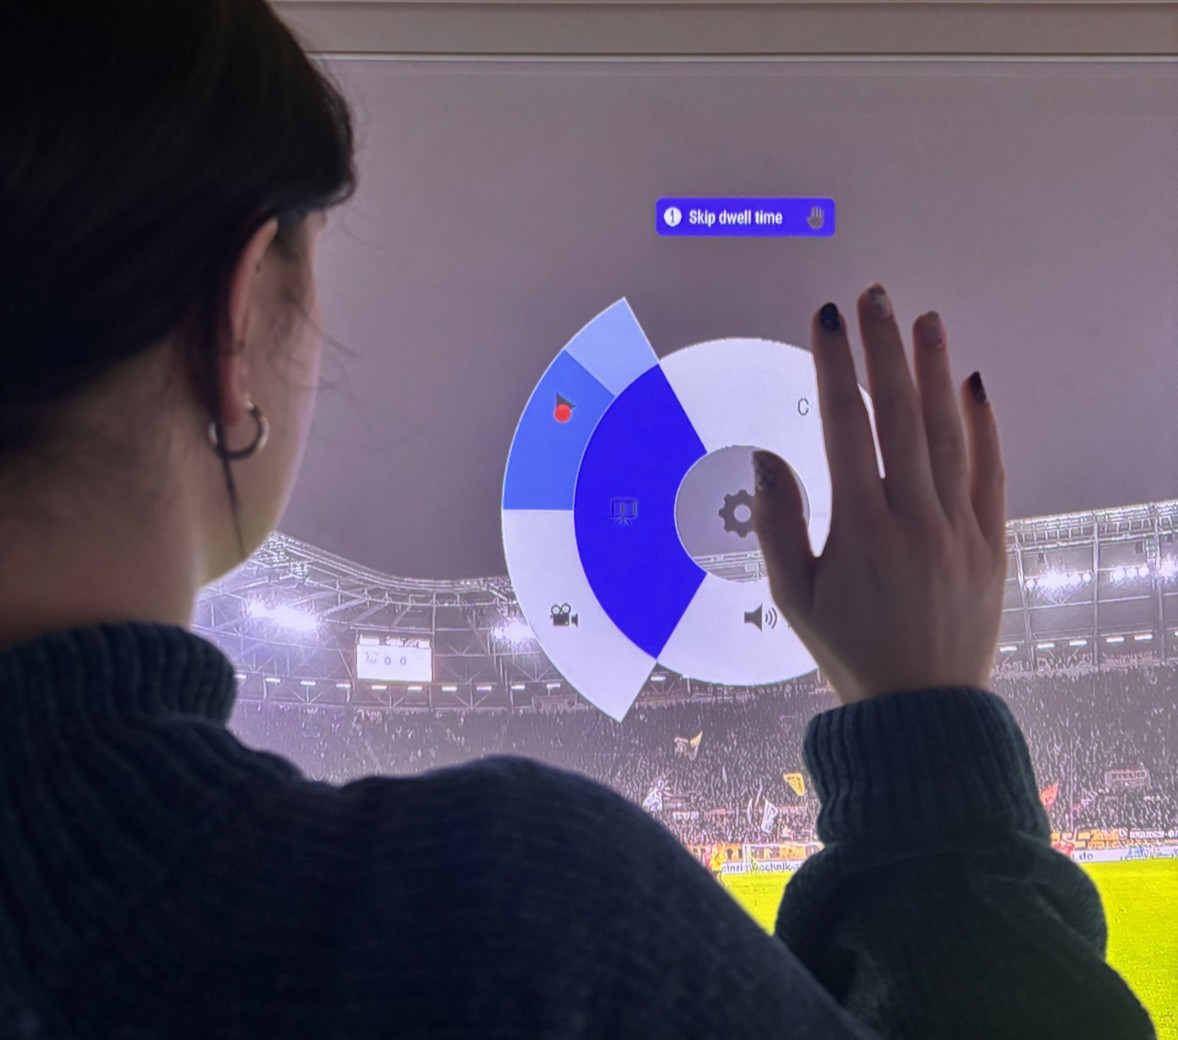
\includegraphics[width=\linewidth]
        {content/images/photo_mir1.jpg}
        \caption{Nutzerin hovert Play Button.}
        \label{fig:photo_mir1}
    \end{subfigure}
    \hfill
    \begin{subfigure}[t]{0.32\textwidth}
        \centering
        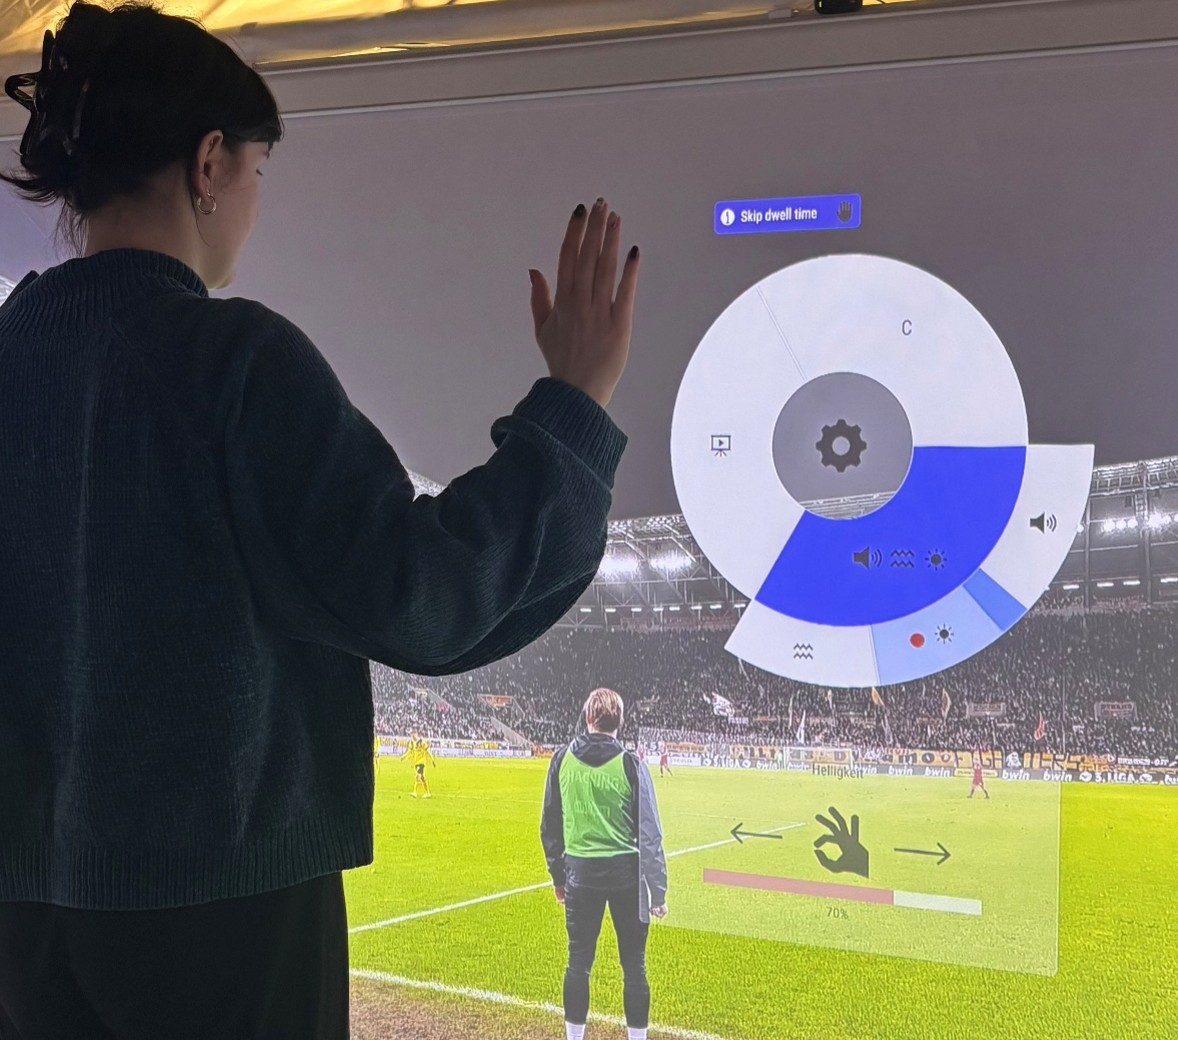
\includegraphics[width=\linewidth]
        {content/images/photo_mir2.jpg}
        \caption{Nutzerin öffnet Vorschau für Helligkeitsslider.}
        \label{fig:photo_mir2}
    \end{subfigure}
    \hfill
    \begin{subfigure}[t]{0.32\textwidth}
        \centering
        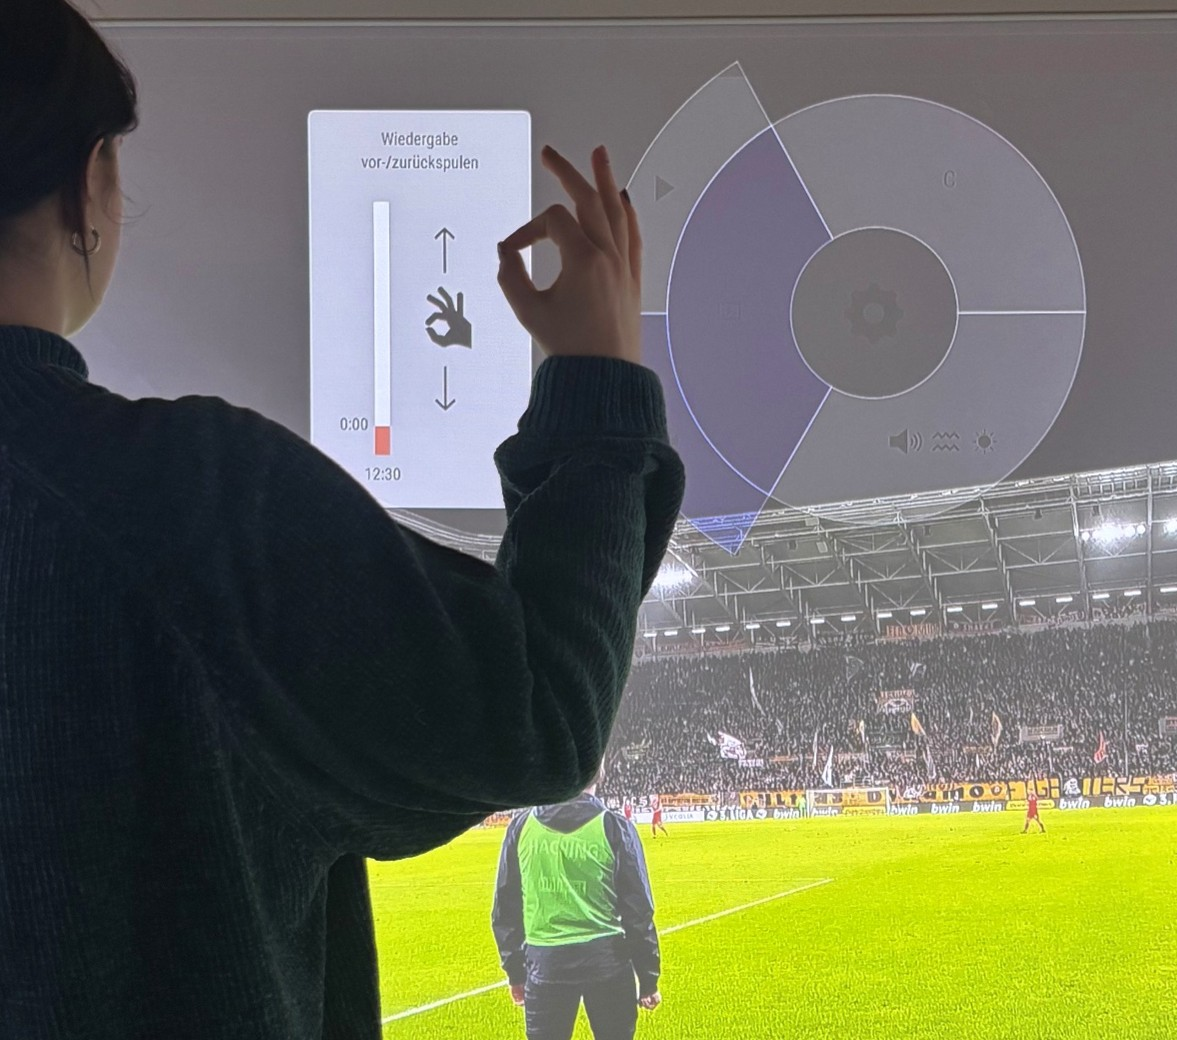
\includegraphics[width=\linewidth]
        {content/images/photo_mir3.jpg}
        \caption{Nutzerin manipuliert Wiedergabezeitpunkt.}
        \label{fig:photo_mir3}
    \end{subfigure}
    \caption{Nutzerin modifiziert Einstellung mit Hilfe von Marking-Menu im MIR. Das ausgewählte Szenario ist das Fußballstadion.}
    \label{fig:photos_mir}
\end{figure}


\subsection{Systemarchitektur}
Die Systemarchitektur basiert auf einer Verarbeitungspipeline, die in eine modulare Frontend-Struktur eingebettet ist. Aus den Kameradaten werden zunächst Handmerkmale extrahiert. Auf Basis dieser Tracking-Daten wird eine Cursorposition im zweidimensionalen Interaktionsraum berechnet. Diese steuert die Benutzungsoberfläche des Systems, die das Marking-Menu sowie weitere Interaktionselemente darstellt.
Aktionen, die aus der Menüinteraktion entstehen, werden anschließend über eine WebSocket-Schnittstelle an eine angebundene Zielanwendung übertragen.
Abbildung~\ref{fig:handtracking_pipeline_diagram} zeigen die grundlegenden Komponenten der Verarbeitungspipeline des Systems von der Kameradatenerfassung bis zur Übertragung der Interaktionsereignisse an die Zielanwendung.

\begin{figure}[htbp]
    \centering
    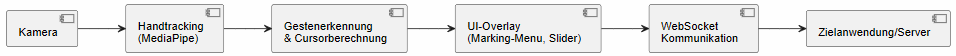
\includegraphics[width=0.99\linewidth]{content/diagrams/handtracking_pipeline_diagram.png}
    \caption{Komponenten der Verarbeitungspipeline des Interaktionssystems}
    \label{fig:handtracking_pipeline_diagram}
\end{figure}

Die Kommunikation zwischen Interaktionssystem und Zielanwendung erfolgt über WebSocket. 
WebSocket ist ein Netzwerkprotokoll, das eine persistente, bidirektionale Kommunikationsverbindung zwischen Client und Server über eine einzelne TCP-Verbindung ermöglicht \parencite{fetteMelnikov2011TheWebsocketProtocol}. Dadurch können Ereignisse in Echtzeit übertragen werden, ohne dass wiederholt neue HTTP-Verbindungen aufgebaut werden müssen.

Neben dieser linearen Verarbeitungskette ist das System in mehrere funktionale Komponenten unterteilt, die innerhalb des Frontends zusammenwirken:
\begin{itemize}
    \item eine Handtracking-Komponente zur Extraktion von Handlandmarken aus Kameradaten,
    \item eine Gestenerkennung und Cursorberechnung zur Ableitung von Interaktions\-zuständen,
    \item ein Datenmodell zur Verwaltung von Menüstruktur und Zustandsinformationen,
    \item eine UI-Steuerung mit Rendering-Komponente zur Darstellung des Marking-Menus und der Interaktionselemente,
    \item sowie eine WebSocket-Kommunikation zur Anbindung externer Zielanwendungen.
\end{itemize}

Abbildung~\ref{fig:component_diagram} zeigt diese Komponenten sowie deren Interaktionen innerhalb des Systems.

\begin{figure}[htbp]
    \centering
    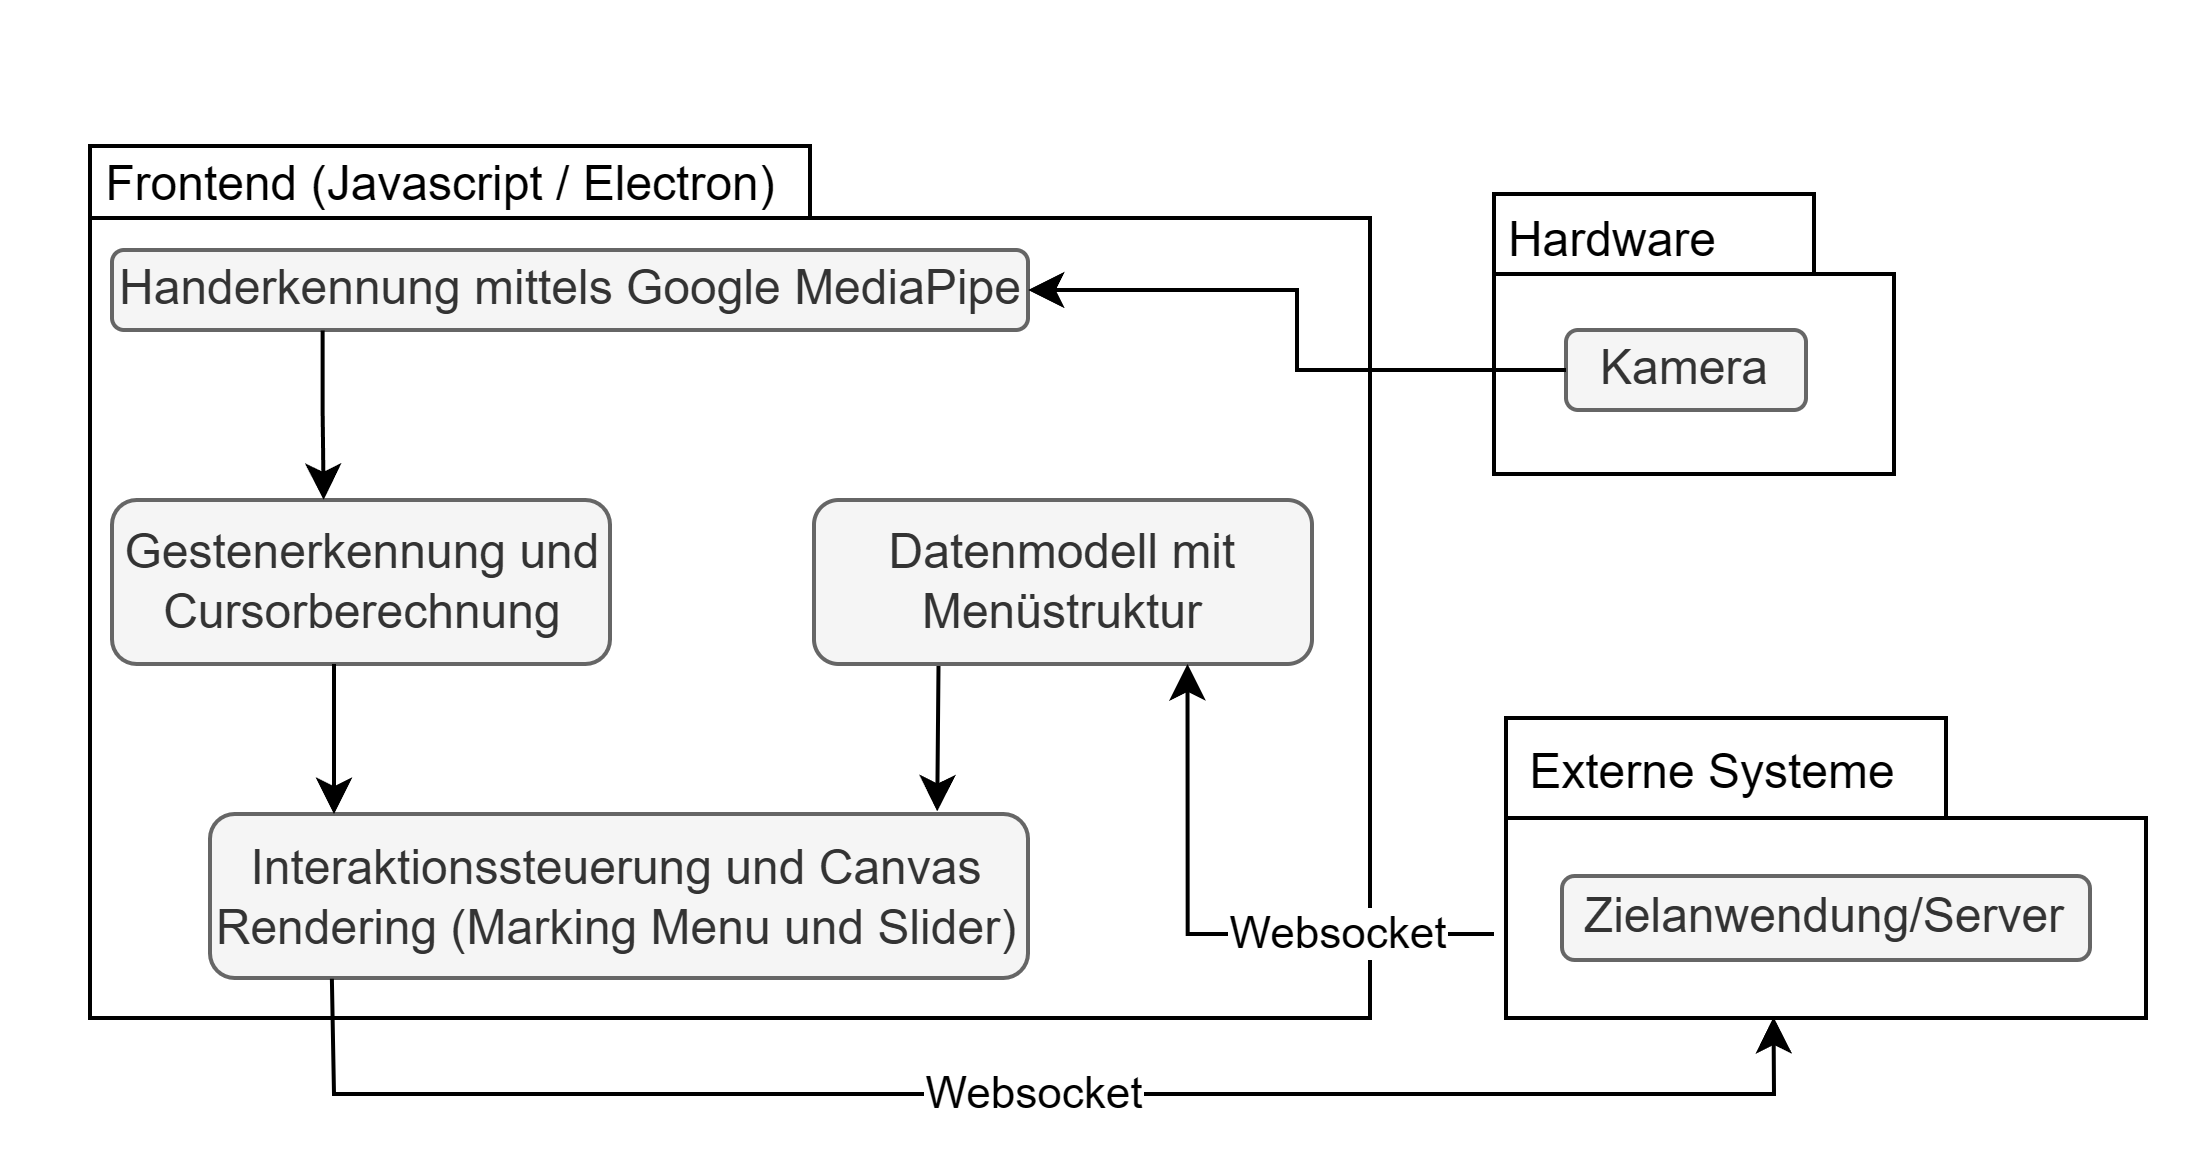
\includegraphics[width=0.8\linewidth]{content/diagrams/component_diagram.png}
    \caption{Vereinfachte Architektur des Interaktionssystems}
    \label{fig:component_diagram}
\end{figure}

Die über WebSocket übermittelten Interaktionsereignisse werden von einer angebundenen Zielanwendung empfangen und verarbeitet. 
Diese Anwendung ist nicht Bestandteil des eigentlichen Interaktionssystems, sondern stellt die Umgebung dar, in der die Interaktionen verarbeitet werden.

Im Kontext des multisensorischen Interaktionsraums wird hierfür typischerweise die \textit{Unreal Engine} verwendet, eine Echtzeit-3D-Engine zur Darstellung und Steuerung der projizierten Inhalte.
Da die Kommunikation jedoch über eine standardisierte Schnittstelle erfolgt, kann das Interaktionssystem prinzipiell mit unterschiedlichen Anwendungen kombiniert werden. 
Dieses Vorgehen unterstützt den Anspruch, das System universell einsetzbar und nicht auf ein einzelnes Anwendungsszenario beschränkt zu gestalten (siehe R2 in Tabelle \ref{tab:requirements}).


\subsection{Handtracking-Pipeline}
\label{sec:handtracking-pipeline}
Die Handtracking-Pipeline bildet die Grundlage des gesamten Interaktionssystems. Ziel ist es, aus dem Kamerabild robuste Informationen über die Position und Form der Hand zu gewinnen und daraus Interaktions\-zustände abzuleiten. Die Implementierung basiert auf einer browsernahen Verarbeitung, sodass die erkannten Handdaten direkt für die visuelle und funktionale Steuerung des Interaktionssystems genutzt werden können.

Zunächst erfasst das System fortlaufend Videoframes der Kamera und übergibt diese an die Handtracking-Komponente \textit{Google MediaPipe}. MediaPipe ist ein Open-Source-Framework zur Echtzeitverarbeitung visueller Sensordaten und stellt vortrainierte Modelle zur Erkennung von Körper-, Gesichts- und Handlandmarken bereit \parencite{lugaresi2019GoogleMediaPipe}. Für jede erkannte Hand liefert das verwendete \textit{MediaPipe Hands Model} 21 dreidimensionale Landmarken, welche die räumliche Lage relevanter Handpunkte beschreiben (siehe Abbildung \ref{fig:mediapipe}).
MediaPipe wurde gewählt, da das Framework eine robuste Echtzeiterkennung von Handlandmarken ermöglicht und direkt in browserbasierten Anwendungen eingesetzt werden kann, wodurch sich die Trackingdaten ohne zusätzliche Verarbeitungsschritte in das Interaktionssystem integrieren lassen.
Auf Basis dieser Landmarken bestimmt das System, ob eine Hand erkannt wurde und welche grundlegende Handhaltung vorliegt.

\begin{figure}[H]
    \centering
    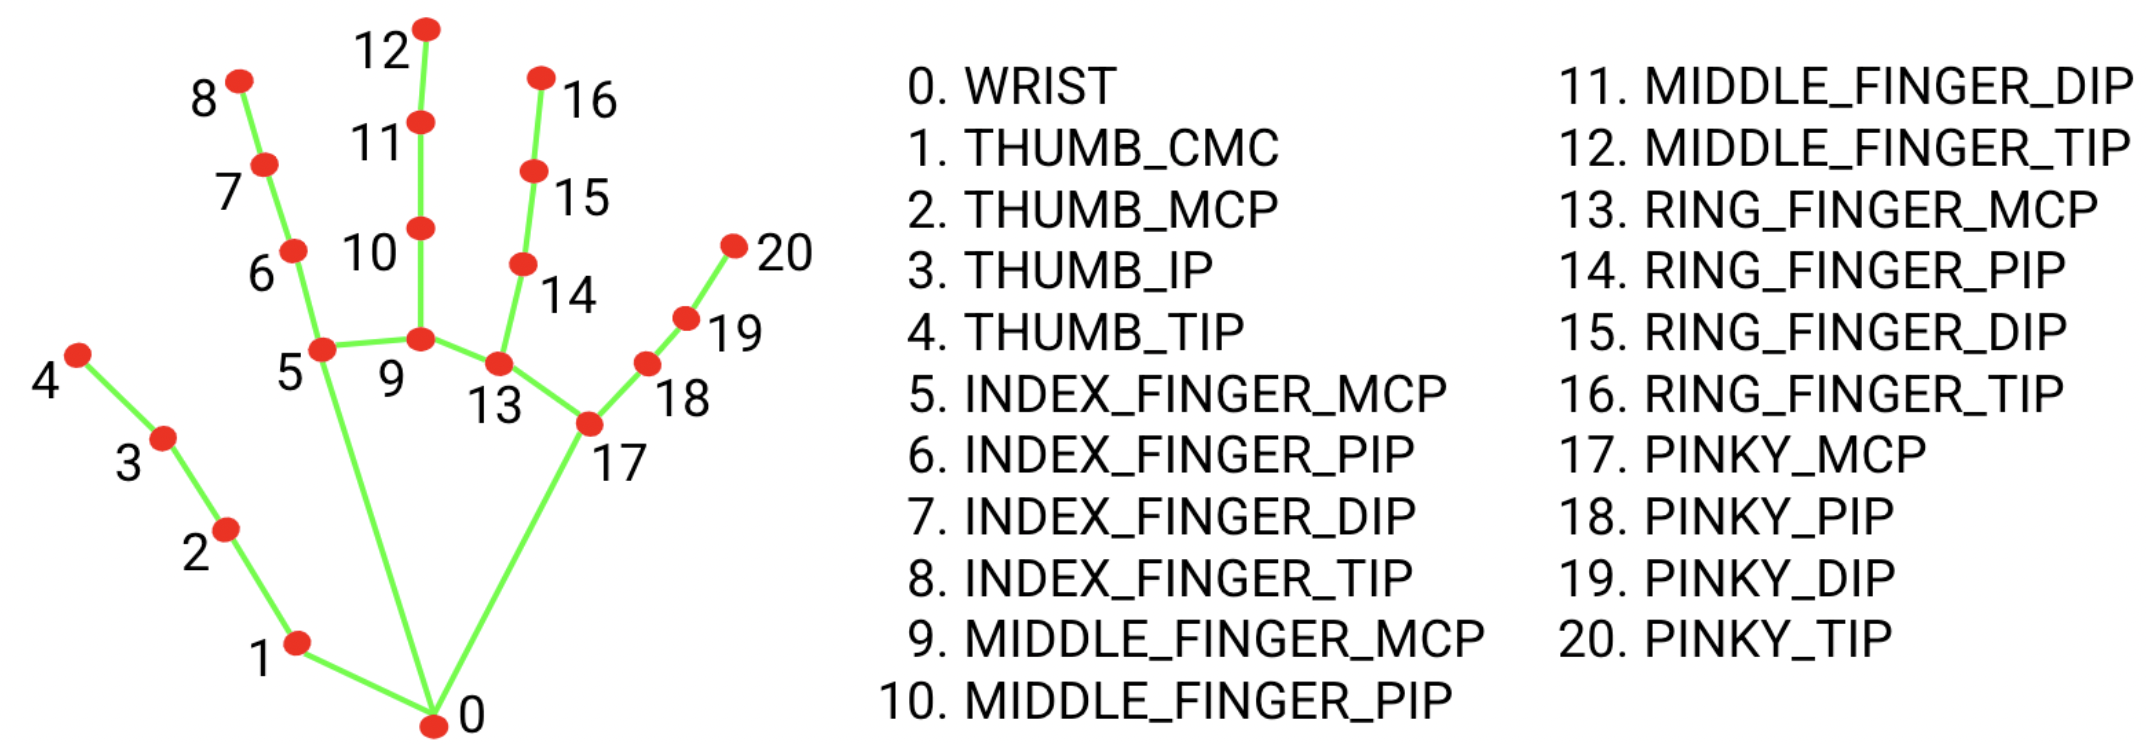
\includegraphics[width=0.9\linewidth]{content/images/mediapipe_landmarks.png}
    \caption{Hand-Landmarken-Modell nach Google MediaPipe \parencite{imageMediapipe_hand_landmarker}}
    \label{fig:mediapipe}
\end{figure}

Ein zentraler Schritt besteht anschließend in der Überführung der Trackingdaten in eine zweidimensionale Cursorposition. Hierfür wird die Handposition auf den Bildschirmraum abgebildet. Der resultierende Cursor dient als primäres Eingabeelement für die Menüinteraktion. Dadurch entsteht eine direkte Kopplung zwischen Handbewegung im Kamerabild und Navigation innerhalb des Intreaktionssystems.
Neben der Positionsbestimmung erfolgt auch die Erkennung diskreter Gesten, wie in Abschnitt~\ref{sec:synthese_konzeption_des_interaktionssystems} erwähnt. Verwendet werden eine offene Hand zur Aktivierung der Menüinteraktion, eine Grab-Geste zur schnellen Bestätigung, sowie eine Pinch-Geste zur kontinuierlichen Steuerung von Slidern. Die Gestenerkennung basiert auf Distanzmaßen zwischen ausgewählten Landmarken (visualisiert in Abbildung \ref{fig:gesture_images_photos}), beispielsweise zwischen Fingerspitzen und Handbasis oder zwischen Daumen und Zeigefinger. Diese Heuristiken ermög\-lichen eine einfache, nachvollziehbare und in Echtzeit ausführbare Klassifikation.  Die erkannten Gesten dienen anschließend als Eingaben für eine zustandsbasierte Interaktionslogik, welche das Verhalten des Menüs steuert.
%Bei der Geste zur Aktivierung wurde zusätzlich darauf geachtet, dass die Geste nur bei frontaler Erkennung ausgelöst wird, um sicherzustellen, dass nur die Kamera an der aktuell frontalen Projektionsfläche das Menü aktivieren kann.

\begin{figure}[H]
\centering
\begin{subfigure}[t]{0.32\textwidth}
    \centering
    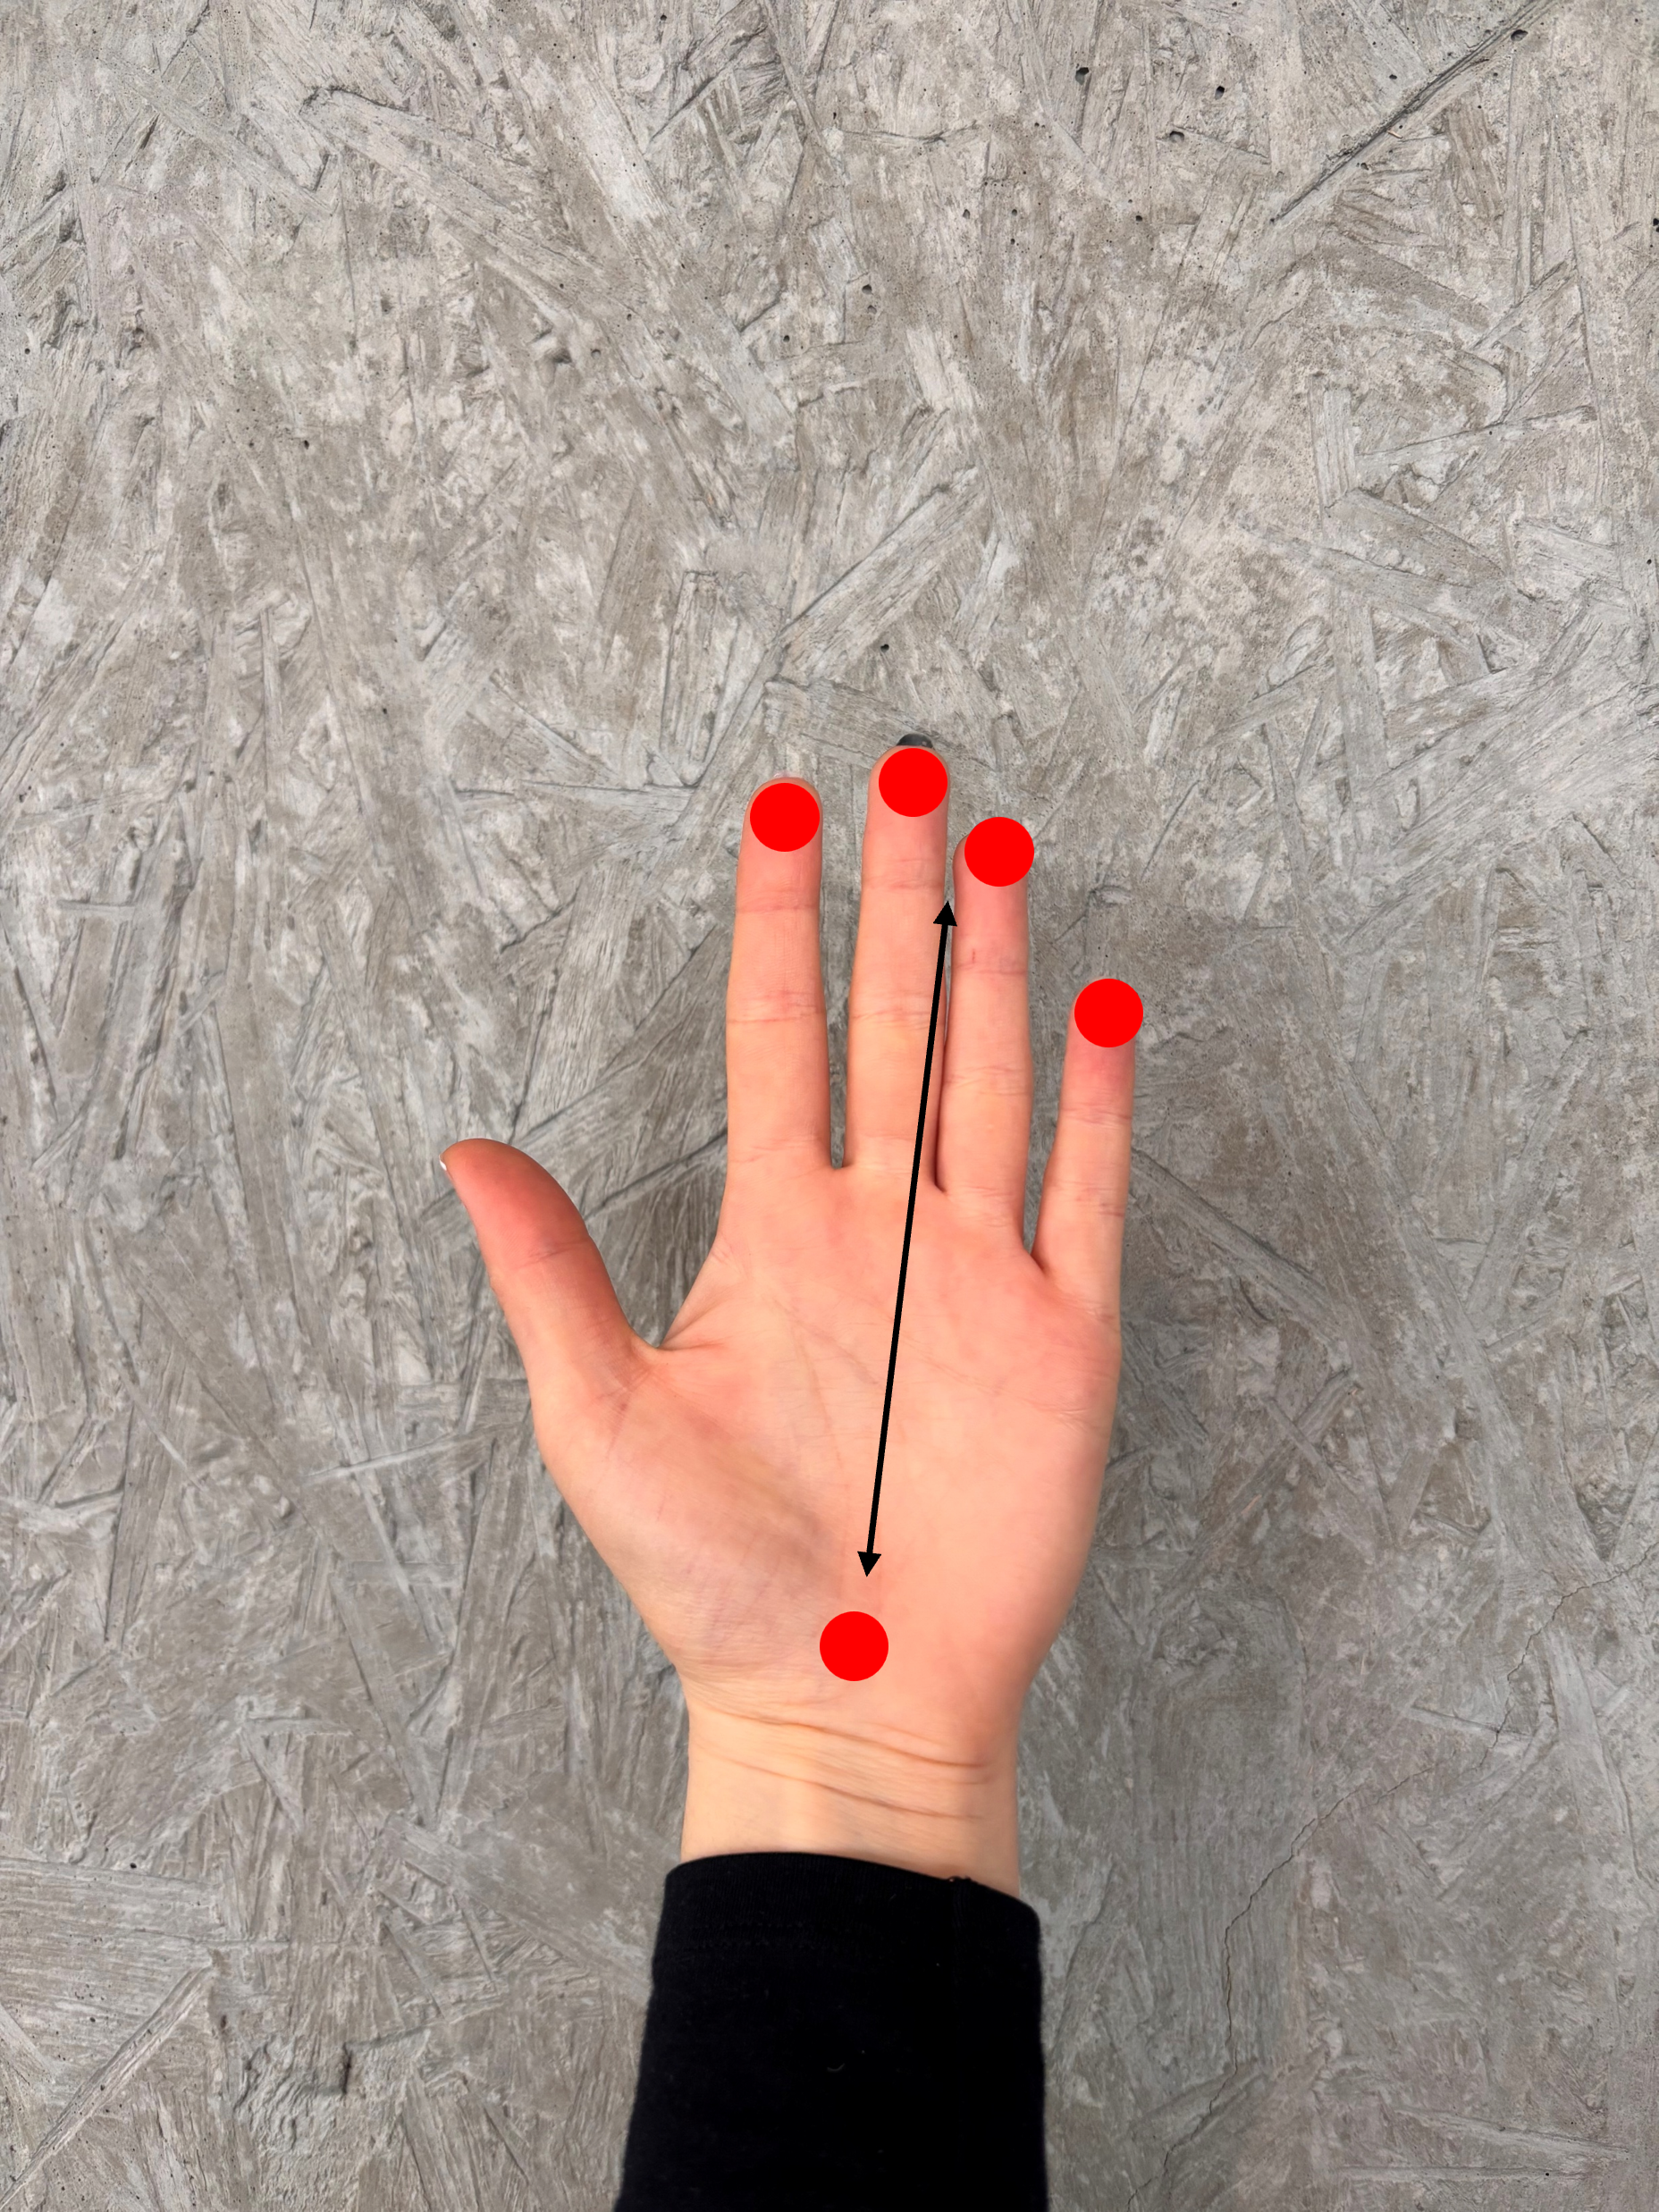
\includegraphics[width=\linewidth]
    {content/images/open_palm_gesture_image.png}
    \caption{Open-Palm-Geste nutzt den Abstand von allen Finger\-spitzen (außer Daumen) und der Handballenunterseite, sowie Spitze von Daumen und kleinem Finger}
    \label{fig:openpalm_gesture_image}
\end{subfigure}
\hfill
\begin{subfigure}[t]{0.32\textwidth}
    \centering
    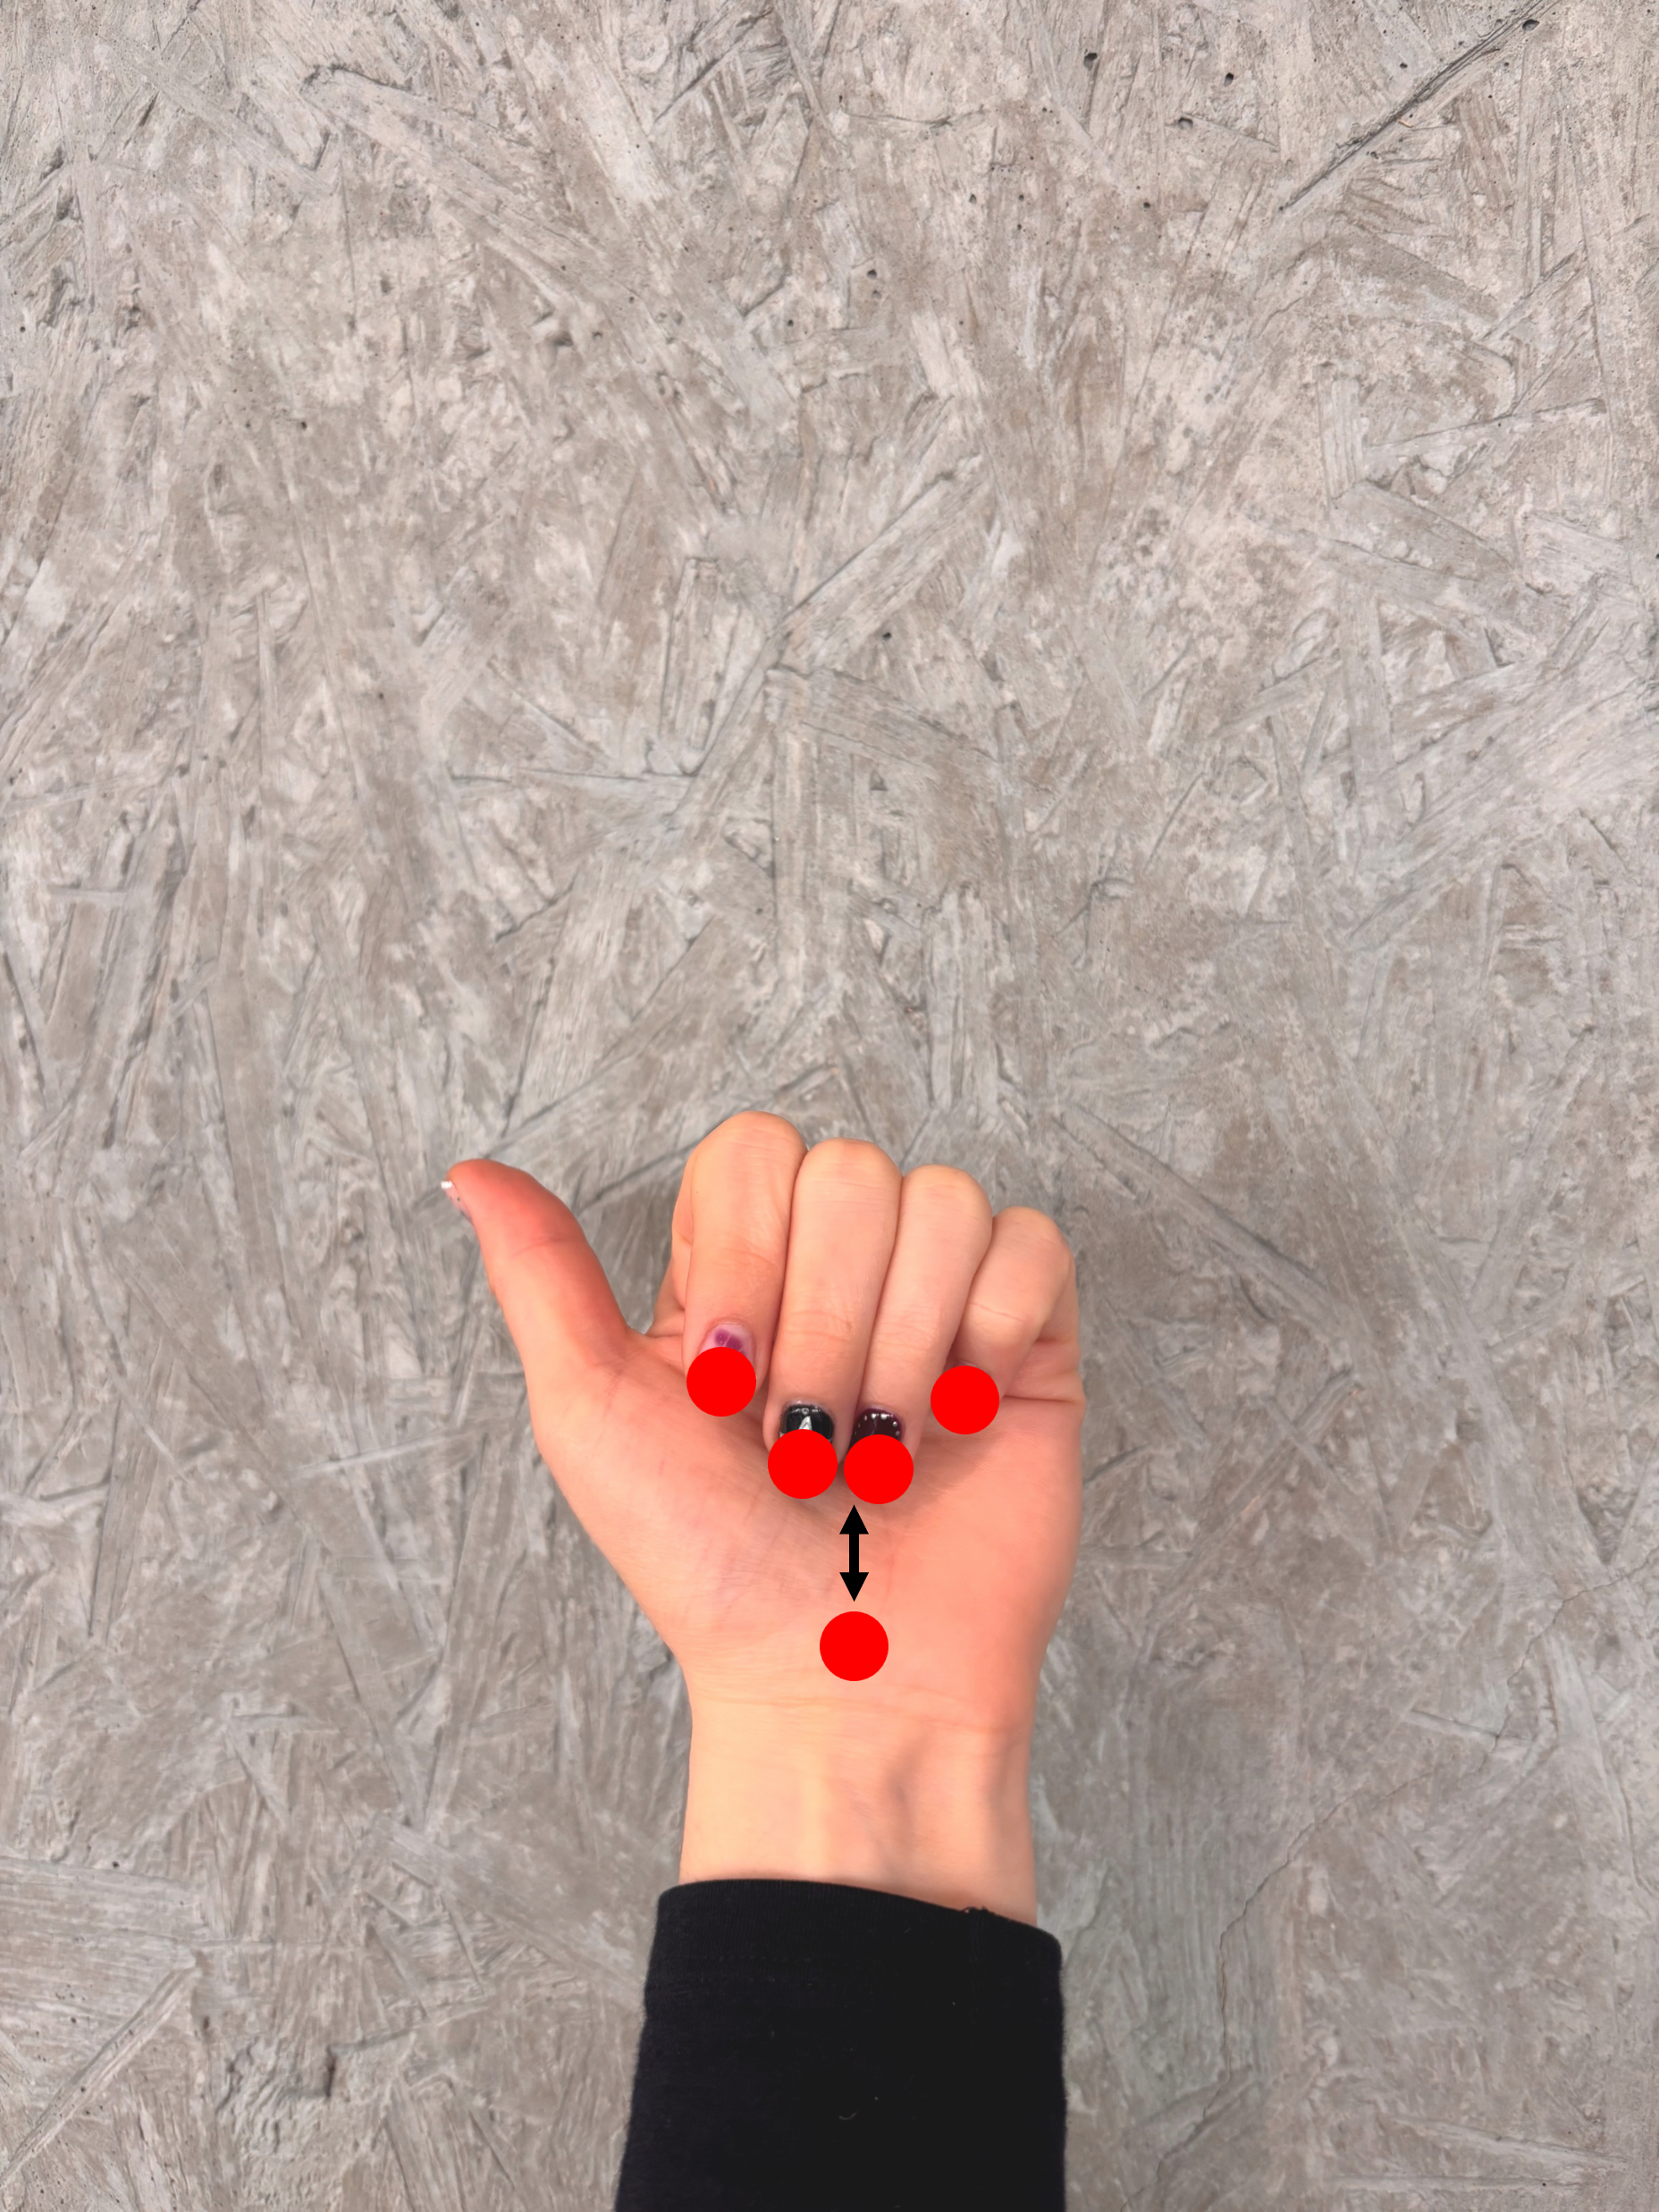
\includegraphics[width=\linewidth]
    {content/images/grab_gesture_image.png}
    \caption{Grab-Geste nutzt den Abstand zwischen allen Fingerspitzen (außer Daumen) und der Handballenunterseite}
    \label{fig:grab_gestute_image}
\end{subfigure}
\hfill
\begin{subfigure}[t]{0.32\textwidth}
    \centering
    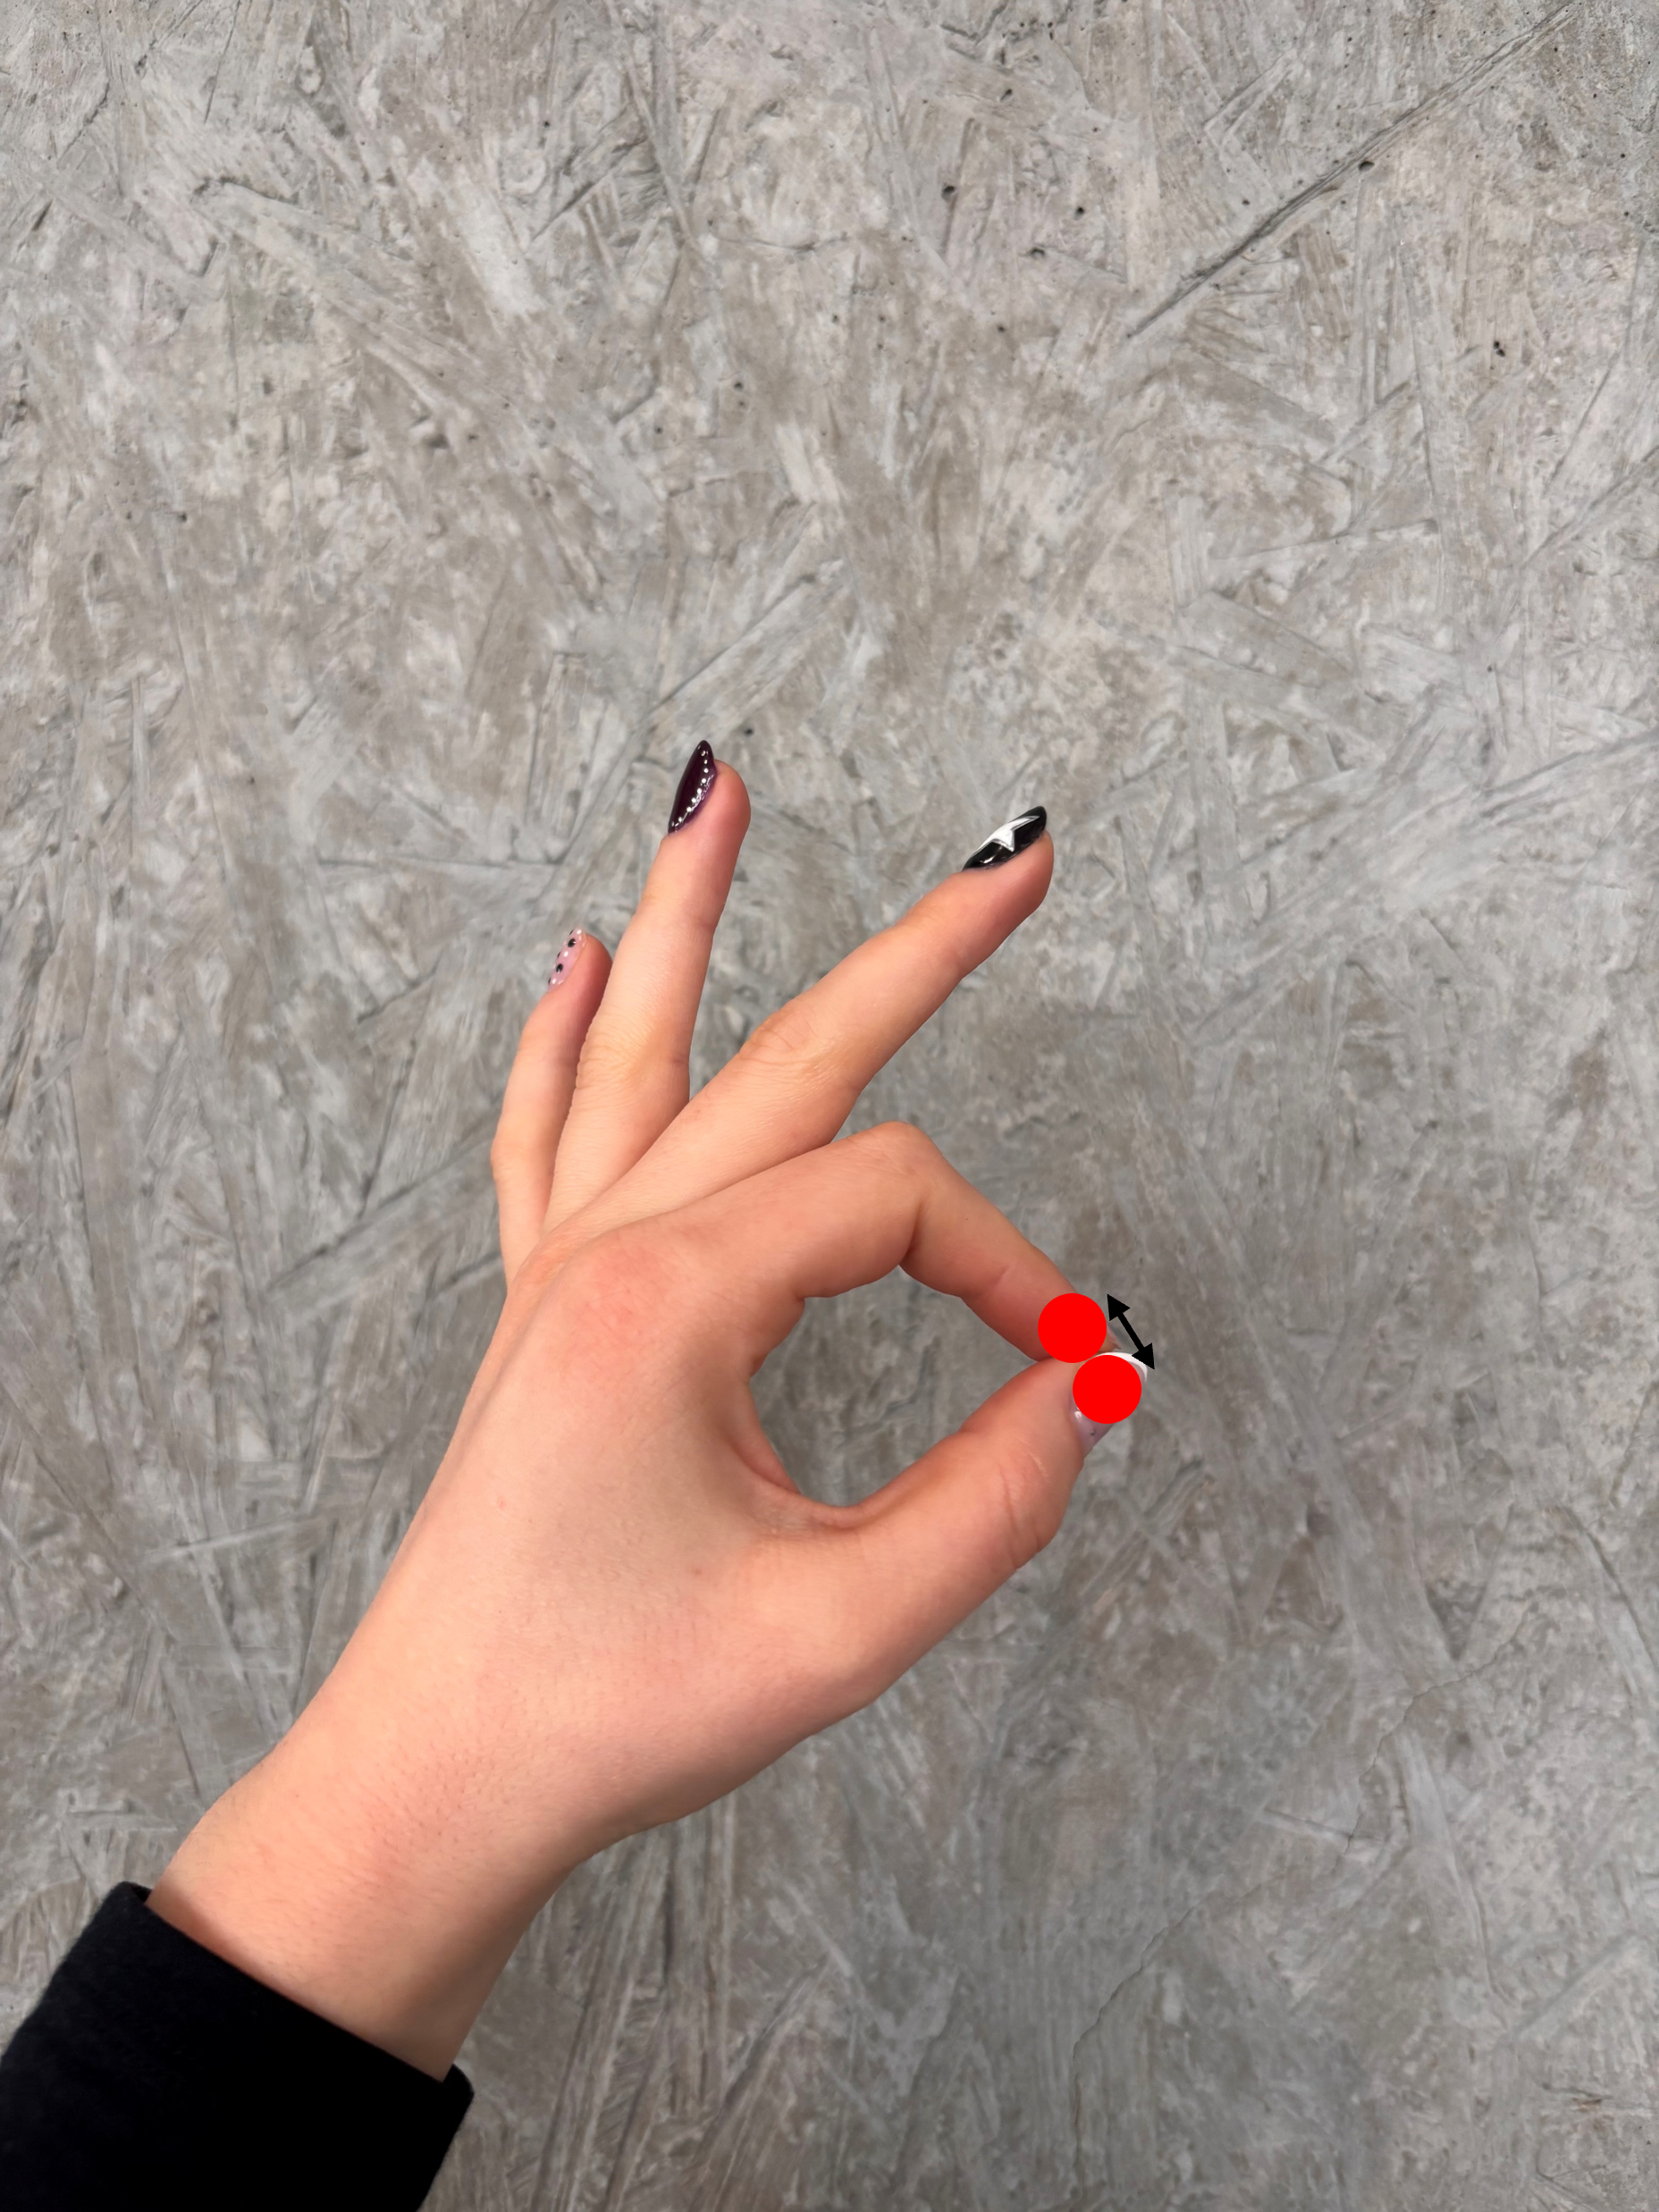
\includegraphics[width=\linewidth]
    {content/images/pinch_gesture_image.png}
    \caption{Pinch-Geste nutzt den Abstand zwischen der Zeigefingerspitze und Daumenspitze}
    \label{fig:pinch_gesture_image}
\end{subfigure}
\caption{Verwendete Gesten und die jeweils zur heuristischen Erkennung herangezogenen Landmarken bzw. Distanzbeziehungen (dargestellt in rot).}
\label{fig:gesture_images_photos}
\end{figure}

Die Handtracking-Pipeline ist eng mit einer Zustandslogik gekoppelt, die den Ablauf der Interaktion steuert (siehe Abbildung~\ref{fig:state_flow_diagram_alt}). Dabei lassen sich mehrere Zustände unterscheiden, die abhängig von der Handerkennung und dem Interaktionsverhalten der Nutzer:innen durchlaufen werden.
Im Ausgangszustand \textit{Activation} ist kein Menü sichtbar. Wird eine Hand erkannt, kann durch Ausführen der Aktivierungsgeste ein Übergang in den Aktivierungsprozess initiiert werden. Wird diese Geste über eine Dauer von drei Sekunden stabil erkannt, wird sie bestätigt und das Menü eingeblendet. Dadurch wird verhindert, dass zufällige oder kurzzeitige Erkennungen unmittelbar zu einer Interaktion führen.
Nach erfolgreicher Aktivierung wechselt das System in den Zustand \textit{Menu}, in dem das Menü sichtbar ist und aktiv genutzt werden kann. Solange eine Hand erkannt wird, bleibt dieser Zustand bestehen und ermöglicht die Interaktion mit den Menüelementen.
Wird keine Hand mehr erkannt, wechselt das System in den Zustand \textit{Idle}, in dem das Menü weiterhin sichtbar bleibt, jedoch keine aktive Interaktion erfolgt. Wird innerhalb dieses Zustands erneut eine Hand erkannt, kehrt das System in den Menüzustand zurück.
Bleibt die Handerkennung für einen längeren Zeitraum aus (mehr als drei Sekunden), wird ein Dwell-Mechanismus ausgelöst, der in den Zustand \textit{Dwell} führt. In diesem Zustand verblasst das Menü visuell, während ein Timer abläuft. Wird innerhalb dieser Phase keine neue Interaktion initiiert, kehrt das System schließlich in den Ausgangszustand \textit{Activation} zurück, in dem das Menü nicht mehr sichtbar ist.
Der Fortschritt der Aktivierung sowie der Übergang in den Dwell-Zustand werden jeweils durch visuelles Feedback im Overlay des Inter\-aktions\-systems vermittelt, sodass Nutzer:innen den aktuellen Interaktionsstatus jederzeit nachvollziehen können.

\begin{figure}[H]
    \centering
    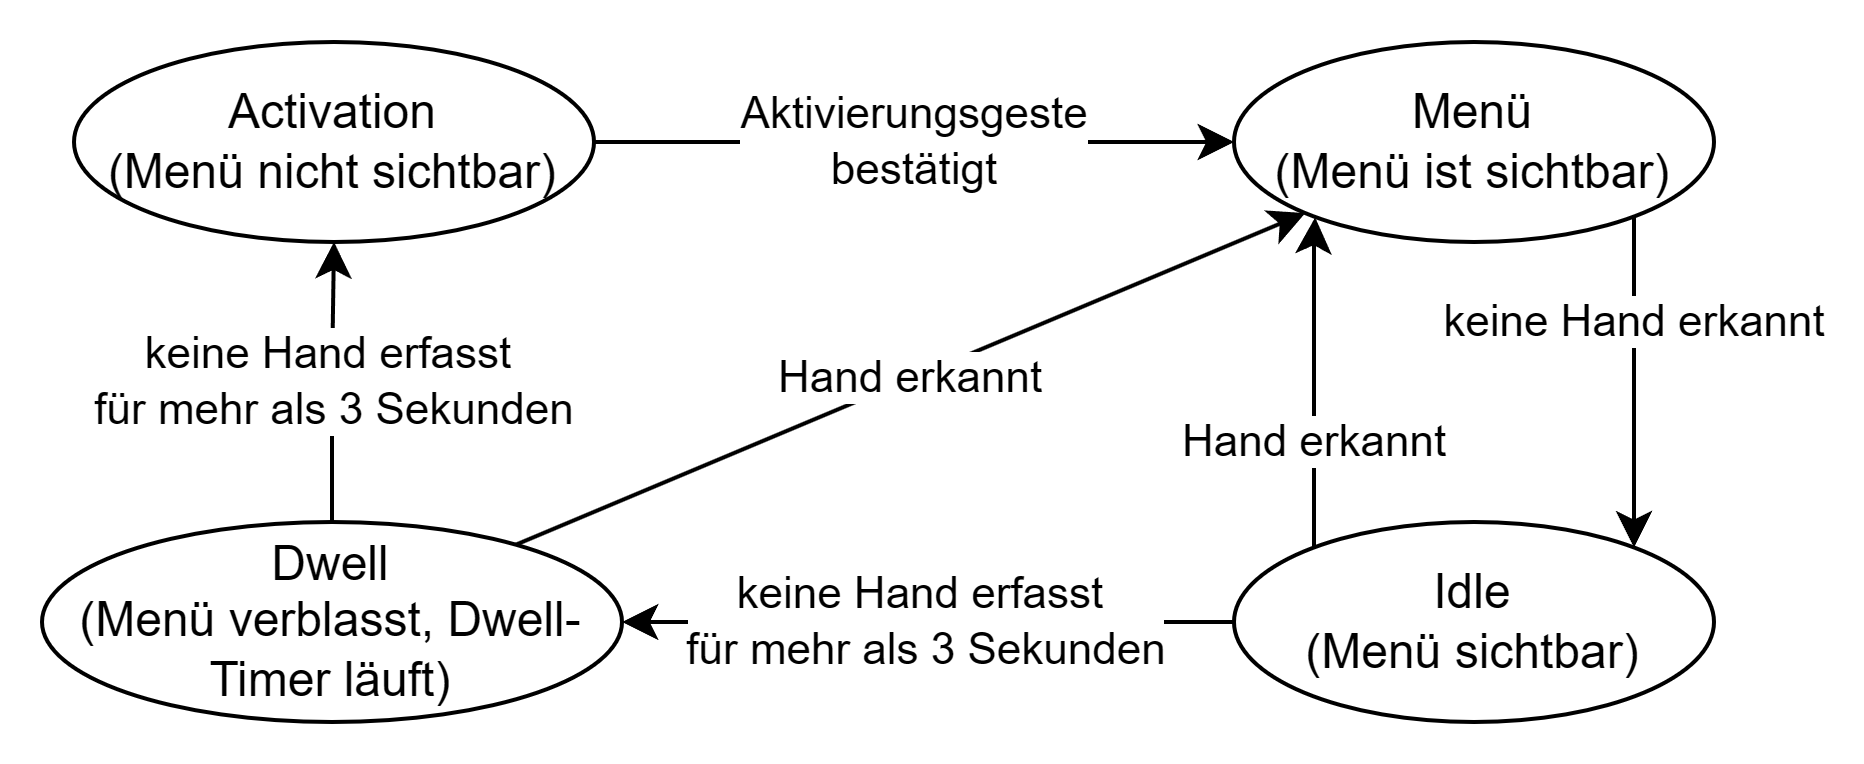
\includegraphics[width=0.8\linewidth]{content/diagrams/state_flow_diagram_alt}
    \caption{Visuali\-sierung der Interaktions\-zustände.}
    \label{fig:state_flow_diagram_alt}
\end{figure}


\subsection{Electron-Overlay}

Die Umsetzung des Interaktionssystems (im als Folgenden \textit{Overlay} bezeichnet, was das gesamte Interaktionssystem einschließlich Benutzungsoverfläche, Interaktionslogik und Kommunikationsschnittstelle umfasst) erfolgt in Form einer modular aufgebauten Electron-Anwendung.
Die Projektstruktur ist so gestaltet, dass Interaktionslogik, Benutzungsoberfläche und Systemintegration klar voneinander getrennt sind.
Listing~\ref{lst:project_structure} zeigt die grundlegende Ordner- und Dateistruktur der Anwendung.
\begin{lstlisting}[
    caption={Projektstruktur der Electron-Anwendung},
    label={lst:project_structure},
    basicstyle=\ttfamily\small
]
gesture-interface/
|-- electron-app/           # Electron-Anwendung
|-- images/                 # UI-Grafiken und Assets
|-- js/                     # Zentrale Interaktionslogik
|   |-- cameraSelector.js   # Kamerakalibrierung
|   |-- cursor.js           # Cursorberechnung
|   |-- data.js             # Datenmodell
|   |-- debugControls.js    # Debugfunktionen
|   |-- gestures.js         # Gestenerkennung
|   |-- main.js             # Einstiegspunkt
|   |-- menu.js             # Menuelogik
|   |-- slider.js           # Slidersteuerung
|   |-- timings.js          # Zustands-Timing
|   `-- websocket.js        # Kommunikation
|-- lib/                    # Externe Bibliotheken (MediaPipe)
|-- index.html              # UI-Struktur
|-- offlineMenu.json        # Menuedefinition
`-- style.css               # Styling
\end{lstlisting}

Die Struktur verdeutlicht die Trennung zwischen der Interaktionslogik im Verzeichnis \texttt{js/},
der visuellen Darstellung über HTML und CSS sowie der Systemintegration durch Electron.
Insbesondere sind Gestenerkennung, Menülogik und Zustandsverwaltung als eigenständige Module implementiert,
was eine klare Strukturierung der Anwendung sowie eine erleichterte Erweiterbarkeit ermöglicht.
Aufbauend auf dieser modularen Struktur wird im Folgenden die technische Umsetzung des Overlays näher erläutert.


\subsubsection{Technische Umsetzung}
\label{sec:technische_umsetzung}
Das visuelle Interaktionssystem wurde als Overlay mit \textit{Electron} umgesetzt.
Electron ist eine Open-Source-Plattform zur Entwicklung plattformübergreifender Desktopanwendungen auf Basis von Webtechnologien \parencite{electronDocumentation}. Anwendungen werden dabei in einer Chromium-Umgebung ausgeführt, also innerhalb einer auf dem Open-Source-Webbrowser Chromium basierenden Laufzeitumgebung, und können gleichzeitig auf systemnahe Funktionen zugreifen.
Die Wahl von Electron ermöglicht eine flexible und plattformunabhängige Implementierung der Benutzungsoberfläche, wodurch das Overlay unabhängig von der jeweiligen Zielanwendung ausgeführt werden kann.
Electron wird dabei als eigenständiger UI-Layer genutzt, der unabhängig von der jeweils gesteuerten Anwendung arbeitet. Diese Trennung ist wesentlich, da das Menü nicht als Bestandteil einer konkreten Zielanwendung implementiert werden soll.
Durch diese Architektur kann das Interaktionssystem als zusätzliche Steuerungsschicht über bestehende Anwendungen gelegt werden, ohne dass diese selbst angepasst werden müssen.


\subsubsection{Visuelle Darstellung und Rückmeldungen}
Das Interaktionssystem wird als transparentes Overlay über der eigentlichen Anwendung dargestellt. Innerhalb dieses Overlays werden sämtliche visuellen Elemente der Interaktion gerendert, ohne die Darstellung der zugrunde liegenden Anwendung zu verdecken. Dabei ist das Fenster standardmäßig nicht fokussierbar, sodass Tastatureingaben weiterhin an die darunterliegende Anwendung weitergeleitet werden können. Dies ist insbesondere relevant, da die Zielanwendung in vielen Szenarien parallel über klassische Eingabegeräte steuerbar bleiben soll.

Innerhalb des Overlays werden das Marking-Menu, der Cursor, visuelle Statusanzeigen sowie kontextabhängige Steuerelemente wie Slider dargestellt. Die Darstellung folgt den in Abschnitt~\ref{sec:synthese_visual_feedback} beschriebenen Gestaltungsentscheidungen und setzt diese technisch innerhalb eines Canvas-Elements um.
Da die Handtracking-Pipeline kontinuierlich pro Frame aktualisierte Positions- und Gestendaten liefert, basiert die Darstellung auf einem framebasierten Renderansatz. Das Menü sowie der Cursor werden bei jeder Aktualisierung vollständig neu gezeichnet, sodass zu jedem Zeitpunkt ausschließlich der aktuelle Interaktionszustand sichtbar ist. Dieses Vorgehen ermöglicht eine konsistente und latenzarme Darstellung dynamischer Zustandsänderungen und vereinfacht die Synchronisation zwischen Trackingdaten, Interaktionslogik und visueller Ausgabe.

Für die konkrete Interaktion ist entscheidend, wie die aktuelle Cursorposition einem Menüelement zugeordnet wird. Die Bestimmung des fokussierten Menüelements basiert auf der relativen Position des Cursors zum Zentrum des Menüs. Hierfür wird die Cursorposition in Polarkoordinaten überführt, wobei insbesondere der Winkel und der Abstand zum Menüzentrum berücksichtigt werden. Der Winkel bestimmt, in welches Segment des radialen Menüs der Cursor fällt, während der Abstand verwendet wird, um zwischen den Menüebenen zu unterscheiden. Auf diese Weise kann eindeutig bestimmt werden, welches Menüelement aktuell fokussiert ist. Dieses Verfahren ermöglicht eine kontinuierliche und stabile Zuordnung von Cursorbewegungen zu Menüsegmenten und bildet die Grundlage für die Steuerung des Marking-Menus.

Das Marking-Menu ist datengetrieben implementiert. Die Menüstruktur wird nicht fest in der Oberfläche hinterlegt, sondern zur Laufzeit aus einer externen JSON-Konfiguration geladen, die von der Zielanwendung bereitgestellt wird. Dadurch können Anzahl der Einträge, Hierarchie und zugehörige Aktionen dynamisch angepasst werden, ohne Änderungen an der Benutzeroberfläche vornehmen zu müssen. Der inhaltliche Aufbau sowie die Gestaltung der Interaktionszustände wurden bereits in Abschnitt~\ref{sec:synthese_konzeption_des_interaktionssystems} beschrieben.

Für Entwicklungs- und Konfigurationszwecke kann das Overlay temporär in einen Konfigurationsmodus versetzt werden. In diesem Modus werden Tastatur- und Mauseingaben abgefangen und für Kalibrierungsfunktionen genutzt. Der Konfigurationsmodus wird in Abschnitt~\ref{sec:development} näher erläutert.


\subsubsection{Zustandslogik der Menüinteraktion}
Die Interaktionslogik des Menüs fußt auf einer zustandsbasierten Struktur, die die aktuelle Interaktion der Nutzer:innen mit den Menüelementen abbildet.
Für jede aktive Menüebene (Level) wird ein separater Interaktionszustand verwaltet.
Ein solcher Zustand umfasst Informationen über das aktuell vom Cursor fokussierte Element, das bereits ausgewählte Element sowie den Fortschritt eines Dwell-Timers zur automatischen Auswahl.
Zusätzlich werden Zustandsinformationen wie das zuvor fokussierte Element oder der Status einer aktiven Greifgeste gespeichert.
Die Verwaltung von Interaktions\-zuständen je Level ermöglicht eine konsistente Verarbeitung mehrstufiger Menühierarchien. Eine Visuali\-sierung der Level ist in Abbildung \ref{fig:levels} dargestellt.

\begin{figure}[H]
    \centering
    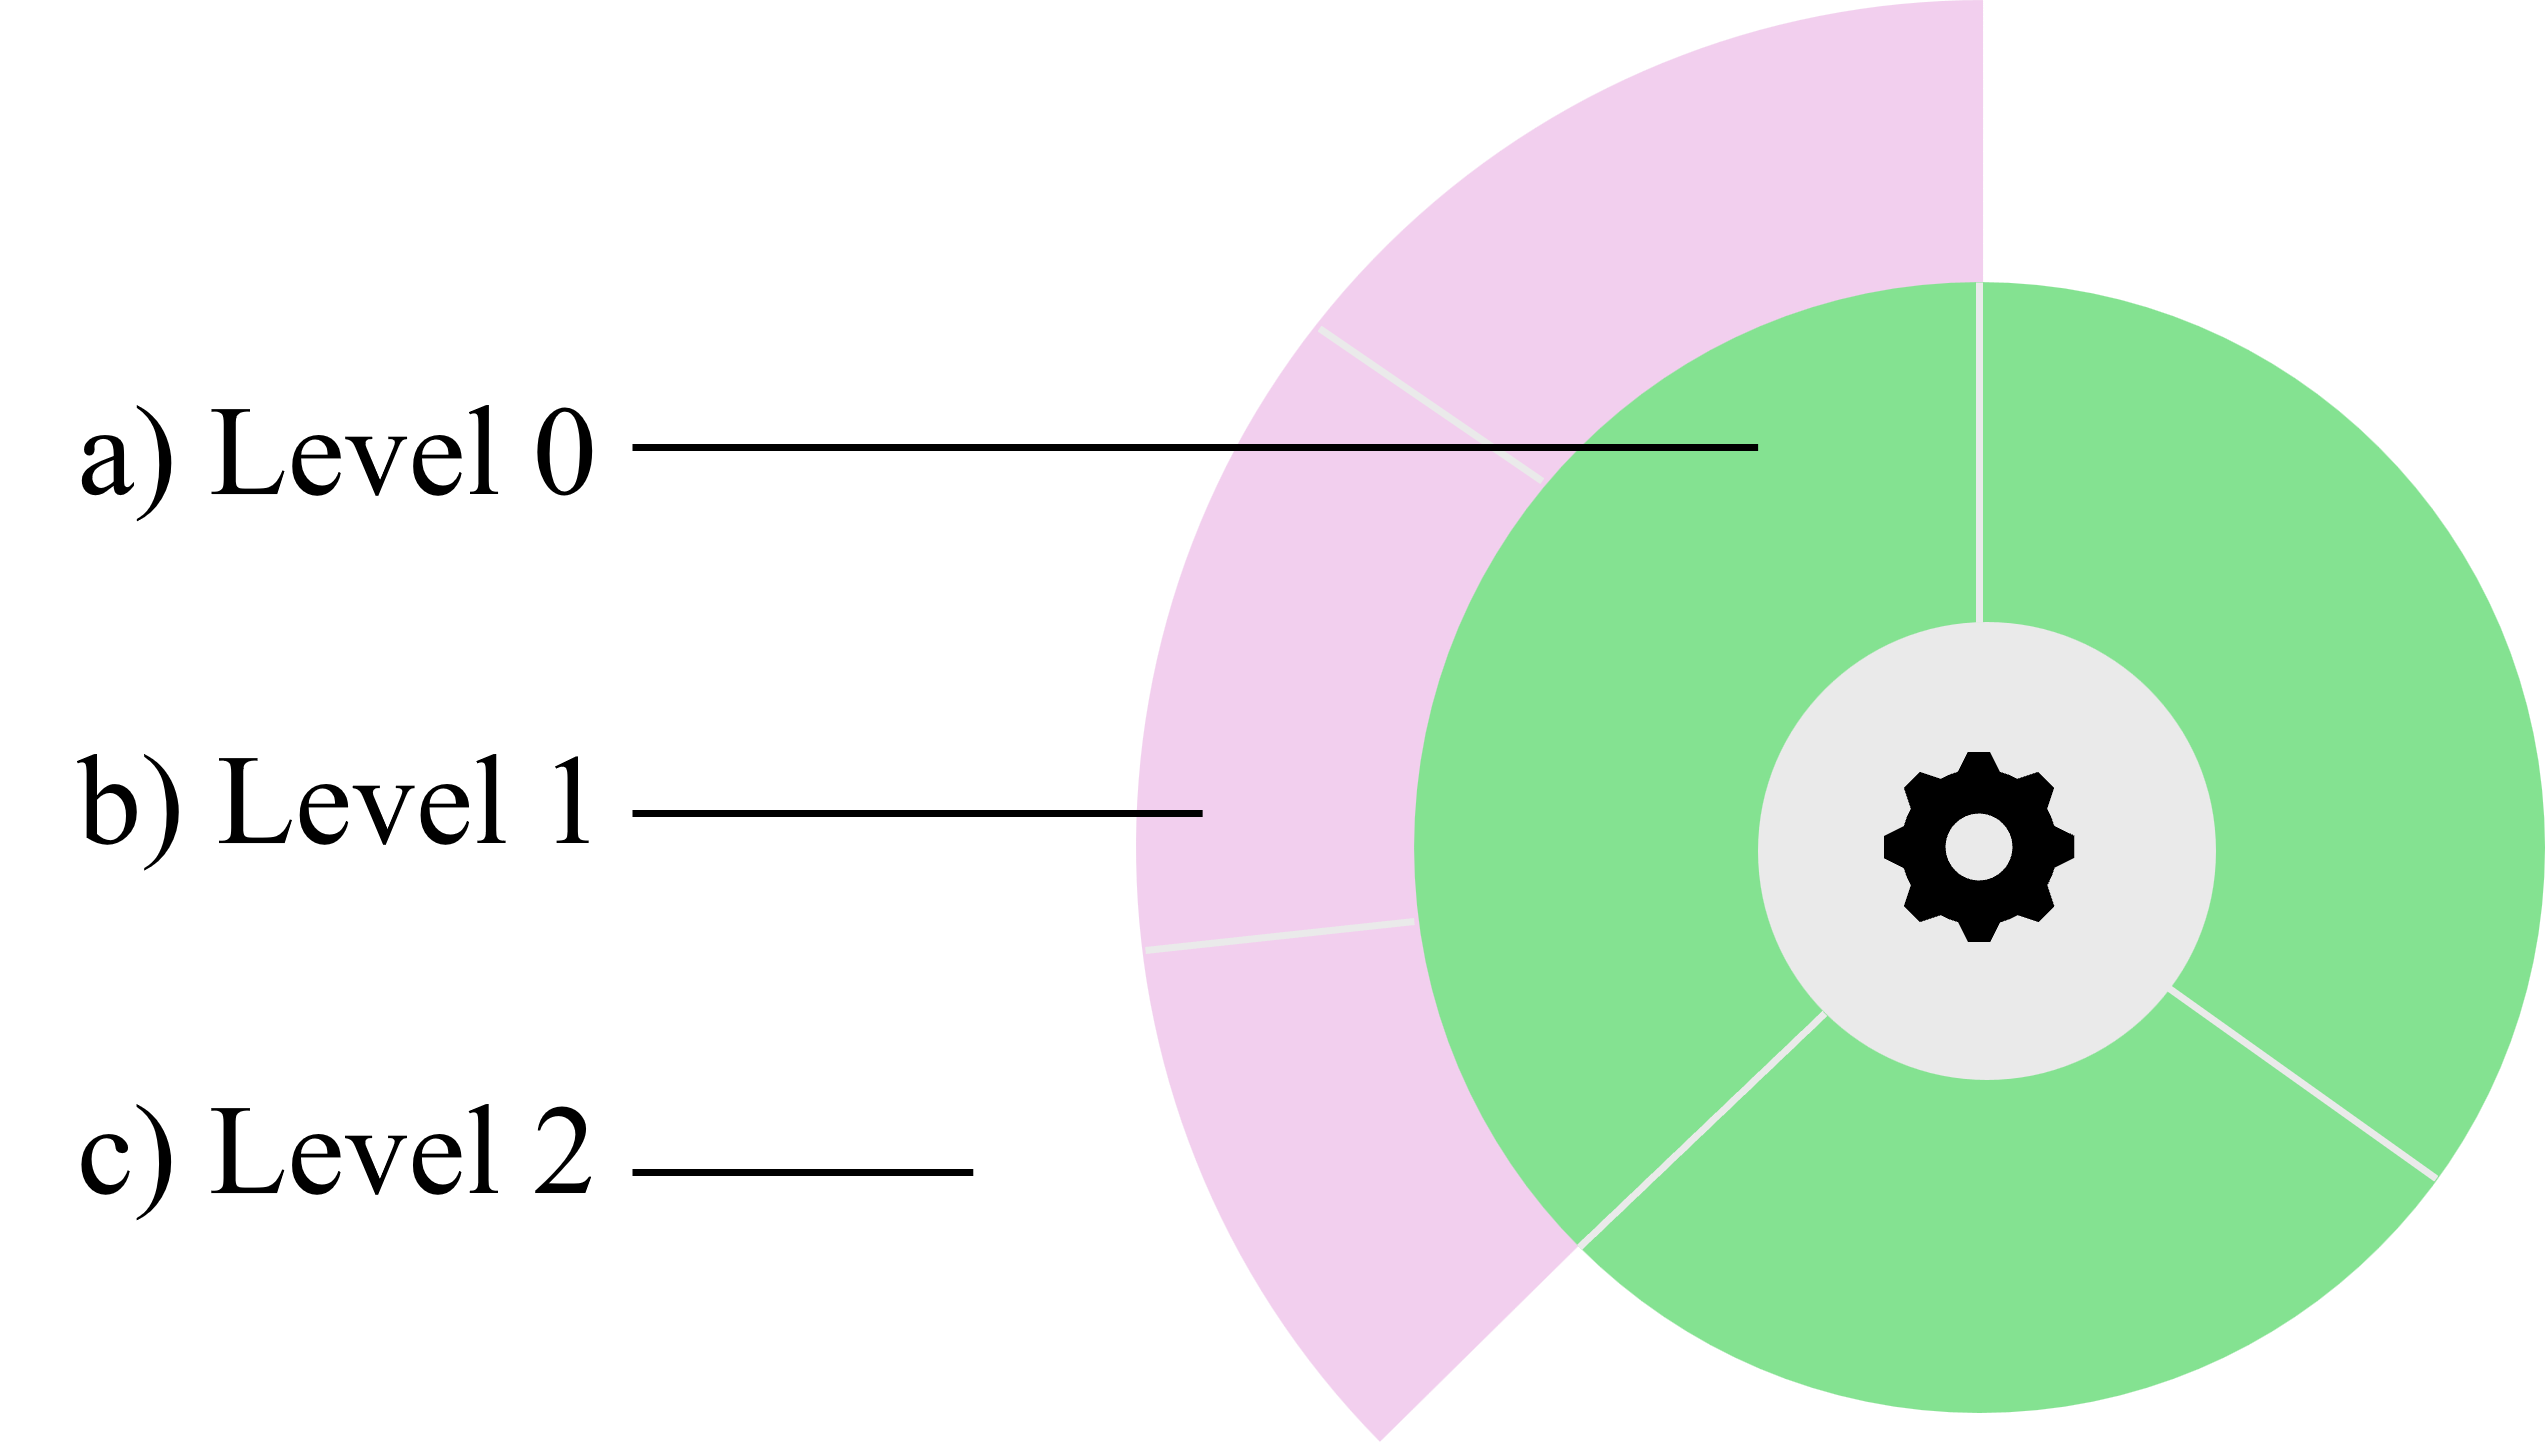
\includegraphics[width=0.45\linewidth]{content/images/levels.png}
    \caption{Visuali\-sierung der Menüebenen (Level) im Menü.}
    \label{fig:levels}
\end{figure}

Für jede Ebene können dadurch unabhängige Hover-, Auswahl- und Dwell-Zustände geführt werden. 
Gleichzeitig unterstützt diese Struktur eine iterative Verarbeitung während des Renderings, da alle aktiven Ebenen sequenziell ausgewertet werden können.


Zur Erkennung von Zustandsänderungen zwischen einzelnen Frames werden zusätzlich vorherige Interaktions\-zustände gespeichert.
Dadurch werden Änderungen wie ein Wechsel des fokussierten Menüelements oder das erstmalige Auftreten einer Greifgeste zuverlässig erkannt.
Diese framebasierte Zustandsverfolgung trägt zu einer möglichst stabilen und konsistenten Interaktionsauswertung bei.

Listing~\ref{lst:levelstates} zeigt beispielhaft eine Funktion zur Erzeugung eines Interaktionszustands für eine einzelne Menüebene. 
Die Funktion gibt ein Zustandsobjekt mit den relevanten Interaktionsparametern zurück und kann entsprechend der Anzahl aktiver Menüebenen mehrfach instanziiert werden.

Die Trennung zwischen globalem Systemzustand (siehe Abschnitt~\ref{sec:handtracking-pipeline}), UI-Zustand und Interaktionszustand verbessert die Erweiterbarkeit des Systems und reduziert Kopplungen zwischen Tracking, Darstellung und Interaktionslogik.
Diese Zustandsstruktur bildet die Grundlage für die Auswertung der Nutzerinteraktionen sowie für die Darstellung der visuellen Rückmeldungen im Menü.

\begin{lstlisting}[language=JavaScript,caption={Beispielhafte Struktur eines Interaktionszustands pro Menüebene},label={lst:levelstates},basicstyle=\ttfamily\footnotesize]
function createLevelState() {
    return {
        // Menuelement, das gerade gehovert wird
        hover: null,
        // Menuelement, das gerade ausgewaehlt ist
        selected: null,
        // Zeitpunkt, zu dem Dwell gestartet ist
        dwellStart: null,
        // Fortschritt des Dwells in Prozent
        dwellProgress: 0,
        // Gibt an, ob dwell bereits getriggert wurde
        dwellTriggered: false,
        // Menuelement, das im letzten Frame gehovert wurde
        previousHover: null,
        // Gibt an, ob Grab-Geste im letzten Frame ausgeloest war
        wasGrabbing: false
    };
}
\end{lstlisting}


\subsection{Datengetriebene Menüstruktur}
Da das im Overlay dargestellte radiale Menü nicht statisch implementiert ist, sondern von der Zielanwendung konfiguriert wird, muss es eine definierte Struktur geben, wie das Menü aufgebaut sein darf. Die Struktur des Menüs wird durch eine JSON-basierte Konfiguration beschrieben, die von der Zielanwendung an das Overlay übermittelt wird. Dadurch kann die Menüstruktur dynamisch angepasst werden, ohne Änderungen an der Benutzungsoberfläche selbst vornehmen zu müssen. Das Overlay ist damit ausschließlich für Darstellung und Interaktionslogik verantwortlich.

Die Konfiguration des Menüs definiert sowohl globale Eigenschaften des Menüs, wie beispielsweise den Radius der Hauptmenüebene oder die Größe von Untermenüs, als auch die einzelnen Menüeinträge.
Ein Menüeintrag kann dabei entweder als Navigationsknoten fungieren, der ein weiteres Untermenü öffnet, oder direkt eine Interaktion auslösen, etwa die Aktivierung eines Buttons oder die Steuerung eines kontinuierlichen Parameters über einen Slider. Dadurch entsteht eine klare Trennung zwischen Navigations- und Aktionsknoten.

Die hierarchische Organisation ermöglicht es, mehrere Interaktionsfunktionen innerhalb einer begrenzten Anzahl sichtbarer Menüsegmente bereitzustellen. 
Während die oberste Ebene zentrale Funktionskategorien enthält, werden detailliertere Steuerungsoptionen innerhalb der entsprechenden Untermenüs zugänglich gemacht.
Jeder Menüeintrag besitzt eine eindeutige Identifikationsnummer (``\texttt{id}'') sowie Metadaten wie eine Bezeichnung (``\texttt{label}''), ein Icon (``\texttt{icon}'') und den Typ des UI-Elements (``\texttt{type}''). Der Typ bestimmt, wie ein Eintrag im Interaktionssystem interpretiert wird, beispielsweise als Untermenü (``\texttt{menu}''), als kontinuierliches Steuerelement (``\texttt{slider}'') oder als diskrete Aktion (``\texttt{button}'').

Abhängig vom Typ des Eintrags können zusätzliche Parameter definiert werden. Eine zentrale Rolle spielt dabei der Schlüssel ``\texttt{target}'', der angibt, welcher Parameter in der Zielanwendung durch die Interaktion beeinflusst wird. Im Fall eines Sliders wird beispielsweise ein kontinuierlicher Wert für den angegebenen Zielparameter übertragen, während bei einem Button diskrete Zustandsänderungen ausgelöst werden. Diese Informationen werden bei der Interaktion als Teil der WebSocket-Nachrichten an die Zielanwendung übermittelt (siehe Abschnitt~\ref{sec:eventcommunication}).

Listing~\ref{lst:menu_config} zeigt beispielhaft eine solche Menükonfiguration. Die oberste Ebene enthält zwei Haupteinträge: ``\texttt{Umgebungseinstellungen}'' und ``\texttt{Presentation}''. Beide Einträge sind vom Typ ``\texttt{menu}'' und enthalten jeweils weitere Untereinträge im Feld ``\texttt{children}''.
Der Eintrag ``\texttt{Umgebungs- einstellungen}'' definiert ein Untermenü mit drei Slidern zur Steuerung von ``\texttt{volume}'', ``\texttt{bright- ness}'' und ``\texttt{vibration}''. Diese entsprechen den globalen Systemparametern.
Der Eintrag ``\texttt{Presen- tation}'' enthält sowohl einen Slider (``\texttt{Timeline}'') zur Steuerung der Wiedergabeposition als auch einen Button (``\texttt{Play/Pause}'') zur Steuerung des Abspielzustands. Beide greifen auf denselben Zielparameter ``\texttt{presentation}'' zu, unterscheiden sich jedoch im Interaktionstyp.
Durch diese strukturierte Beschreibung entsteht zur Laufzeit ein hierarchisches radiales Menü, bei dem die oberste Ebene die beiden Kategorien darstellt und weitere Funktionen über Submenüs zugänglich gemacht werden. Die konkrete visuelle Ausprägung dieses Menüs entspricht den zuvor beschriebenen Menüstrukturen (siehe Abschnitt~\ref{sec:synthese_radiales_menü}).

Diese generische Beschreibung der Menüstruktur ermöglicht es dem Interaktionssystem, unabhängig von konkreten Anwendungsszenarien zu bleiben. Neue Funktionen oder zusätzliche Menü\-ebenen können ergänzt werden, ohne die Implementierung des Overlays selbst zu verändern. Auf diese Weise kann für jedes Anwendungsszenario eine spezifische Menüstruktur definiert werden.

\begin{lstlisting}[language=json,caption={Beispiel einer Menükonfiguration},
label={lst:menu_config},basicstyle=\ttfamily\footnotesize]
{
  "radius": 200,
  "subRadius": 100,
  "items": [
    {
      "id": 1,
      "label": "Umgebungseinstellungen",
      "type": "menu",
      "icon": "settings",
      "children": [
        {
          "id": 11,
          "label": "Volume",
          "type": "slider",
          "icon": "volume",
          "target": "volume"
        },
        {
          "id": 12,
          "label": "Brightness",
          "type": "slider",
          "icon": "brightness",
          "target": "brightness"
        },
        {
          "id": 13,
          "label": "Vibration",
          "type": "slider",
          "icon": "vibration",
          "target": "vibration"
        }
      ]
    },
    {
      "id": 2,
      "label": "Presentation",
      "type": "menu",
      "icon": "presentation",
      "children": [
        {
          "id": 21,
          "label": "Timeline",
          "type": "slider",
          "icon": "timeline",
          "target": "presentation"
        },
        {
          "id": 22,
          "label": "Play/Pause",
          "type": "button",
          "icon": "play",
          "target": "presentation"
        }
      ]
    }
  ]
}
\end{lstlisting}


\subsection{Eventkommunikation}
\label{sec:eventcommunication}
Die Interaktion mit dem Menü erzeugt Interaktionsereignisse, die an die angebundene Zielanwendung weitergeleitet werden. 
Hierfür wird eine WebSocket-basierte Kommunikation eingesetzt. Die Verwendung einer persistenten WebSocket-Verbindung vermeidet wiederholte Verbindungsaufbauten und reduziert damit Latenzzeiten bei der Übertragung von Interaktionsereignissen.

Über diese Verbindung werden sowohl Aktionen vom Overlay an die Zielanwendung gesendet als auch Initialwerte oder Bestätigungsnachrichten von der Anwendung an das Overlay zurückgegeben.
Damit entsteht eine kontinuierliche Kommunikationsschnittstelle zwischen Interaktionssystem und Anwendung.

\subsubsection{Nachrichtenstruktur}
Die übertragenen Nachrichten folgen einer einheitlichen JSON-Struktur (Tabelle \ref{tab:websocket_message}).
Dieses Schema ermöglicht die Beschreibung unterschiedlicher Interaktionsereignisse (zum Beispiel diskrete Buttonaktionen
oder kontinuierliche Slideränderungen) innerhalb eines einheitlichen Kommunikationsprotokolls.
Das Feld \texttt{action} (im Folgenden \textit{Aktion}) beschreibt das Interaktionsereignis.
Nachrichten mit der Aktion ``\texttt{update}'' werden bei Änderungen kontinuierlicher Werte verwendet, während ``\texttt{pressed}'' diskrete Button-Aktionen beschreibt. Nachrichten mit der Aktion ``\texttt{initial}'' werden für die Initialisierung genutzt und können initiale Sliderwerte oder die Menüstruktur selbst senden. Der Typ (``\texttt{type}'') einer Nachricht gibt an, welches Element die Nachricht ausgelöst hat. ``\texttt{slider}''-Typ Nachrichten gehören immer zur Aktion ``\texttt{update}'', während die ``\texttt{pressed}''-Aktion immer zum Typ ``\texttt{button}'' gehört und ``\texttt{type}'' ``\texttt{menu}'' immer zur Aktion ``\texttt{initial}''. Das ``\texttt{target}'' gibt immer das Ziel oder den Kontext der aktuellen Interaktion an, wie ``\texttt{volume}'' oder ``\texttt{presentation}''. \texttt{value} gibt an, welchen Wert die Aktion aktualisiert hat. Im Falle von Slidern sind das meist Angaben zwischen 0 und 1, für Buttons können es spezifische Klick-Events sein. Die ``\texttt{id}'' gibt an, zu welchem Menüelement die Aktion gehört, was nützlich ist, falls es beispielsweise mehrere Slider mit dem Ziel ``\texttt{volume}'' gibt.
Eine beispielhafte Nachricht ist in Listing \ref{lst:slider_update} dargestellt.

\begin{table}[h]
\centering
\begin{tabular}{lll}
\toprule
Feld & Beschreibung & Mögliche Werte \\
\midrule
action & Art der Interaktion & update, pressed, initial \\
type & Typ des UI-Elements & slider, button, menu \\
target & Zielparameter & volume, brightness, vibration, presentation \\
value & übertragener Wert & 0.0–1.0, play, pause \\
id & ID des Menüeintrags & 1, ... \\
\bottomrule
\end{tabular}
\caption{Übersicht über die Felder, die in einer Nachricht gesendet werden.}
\label{tab:websocket_message}
\end{table}


% Motivation für Wahl
Durch die Verwendung eines generischen Nachrichtenformats bleibt die Kopplung zwischen Interaktionssystem und Zielanwendung gering. Das Overlay übermittelt keine anwendungsspezifischen Methodenaufrufe, sondern abstrahierte Interaktionsereignisse. Dadurch kann das System prinzipiell mit unterschiedlichen Anwendungen kombiniert werden. Zusätzlich können neue Interaktionstypen oder Zielparameter ergänzt werden, ohne die grundlegende Kommunikationslogik verändern zu müssen.

\begin{lstlisting}[
    language=json,
    caption={Beispiel einer Slider-Update-Nachricht. Falls sie vom Overlay gesendet wird, bedeutet das, dass der oder die Nutzer:in den Sliderwert des Lautstärkesliders auf 35\% gestellt hat. Der Slider wurde von einem Menüelement mit der ID 1 geöffnet.},
    label={lst:slider_update},
    basicstyle=\ttfamily\small]
{
  "action": "update",
  "type": "slider",
  "target": "volume",
  "value": 0.35,
  "id": "1"
}
\end{lstlisting}

\subsubsection{Kommunikationsfluss}
Nach dem Aufbau der WebSocket-Verbindung sendet die Zielanwendung zunächst Initialisierungsnachrichten mit Konfigurations- und Zustandsdaten, welche den aktuellen Zustand der Anwendung beschreiben. Diese enthalten sowohl die Menüstruktur des Zielsystems als auch weitere Zustandsinformationen, beispielsweise die Länge eines Videos oder aktuelle Parameterwerte. Das Overlay verwendet diese Informationen, um seine UI-Elemente zu initialisieren und mit dem Zustand der Zielanwendung zu synchronisieren. Während der Interaktion übermittelt das Overlay anschließend Ereignisse, etwa Slideränderungen oder Buttonaktionen, an die Zielanwendung. Diese verarbeitet die eingehenden Nachrichten und sendet aktualisierte Parameterwerte zur Bestätigung des neuen Zustands. Das Overlay empfängt diese erst nach Beendigung der aktiven Aktion (beispielsweise wenn der Slider losgelassen wurde), um konsistentes Überschreiben zu vermeiden.

Der grundlegende Kommunikationsfluss zwischen Overlay und Zielanwendung ist in Abbildung~\ref{fig:communication_flow} dargestellt. Die Abbildung verdeutlicht, dass die Kommunikation nicht nur zur Übertragung von Aktionen dient, sondern auch zur Initialisierung sowie zur Synchronisierung von Zustandsinformationen zwischen beiden Komponenten.

% WIP Diagramm:
%@startuml
%actor User as "Nutzer:in"
%participant UI as "Interaktionssystem/Overlay"
%participant Zielanwendung as "Zielanwendung/Server"
%
%== Verbindungsaufbau==
%UI -> Zielanwendung: WebSocket-Verbindung über Port des Servers
%== Initiale Synchronisation ==
%Zielanwendung-> UI: sende Nachrichten vom Typ "initial"
%note over UI,Zielanwendung
%Menüstruktur
%Beispielhafte initiale Informationen:
%- Aktuelle Werte für Sliderkonfigurationen
%(vibration, volume, brightness: 0..1)
%- Länge des Videos
%end note
%UI -> UI : Werte lokal speichern
%UI -> UI : Slider mit Serverzustand synchronisieren
%
%== Erfolgreiche Interaktion==
%User-> UI : Sliderwert mit Geste ändern
%UI -> UI: Update der visuellen Benutzungsoberfläche
%UI -> Zielanwendung: sendet Nachricht vom Typ "update"
%note right of Zielanwendung
%Empfängt Nachricht und aktualisiert
%interne Werte des target-Typs
%(zum Beispiel Lautstärke)
%end note
%Zielanwendung-> UI : sendet Nachricht mit aktuellen Werten\nals Bestätigung / Synchronisation
%UI -> UI : Werte speichern
%UI -> UI : Sliderwerte und UI aktualisieren
%
%== Interaktionslogik==
%note over UI
%Während des aktiven Verschiebens eines Sliders
%werden lokale Interaktionswerte verwendet.
%Erst nach dem Loslassen wird der Serverwert
%zur Synchronisation übernommen.
%end note
%note over UI,Zielanwendung
%Vorteil:
%- deutlich weniger Nachrichtenverkehr
%- durch Verwendung von lokaln Werten und
%On-Demand Synchronisation spüren
%Nutzer:innen keine Latenz
%end note
%note over UI,Zielanwendung
%end note
%
%@enduml


\begin{figure}
\centering
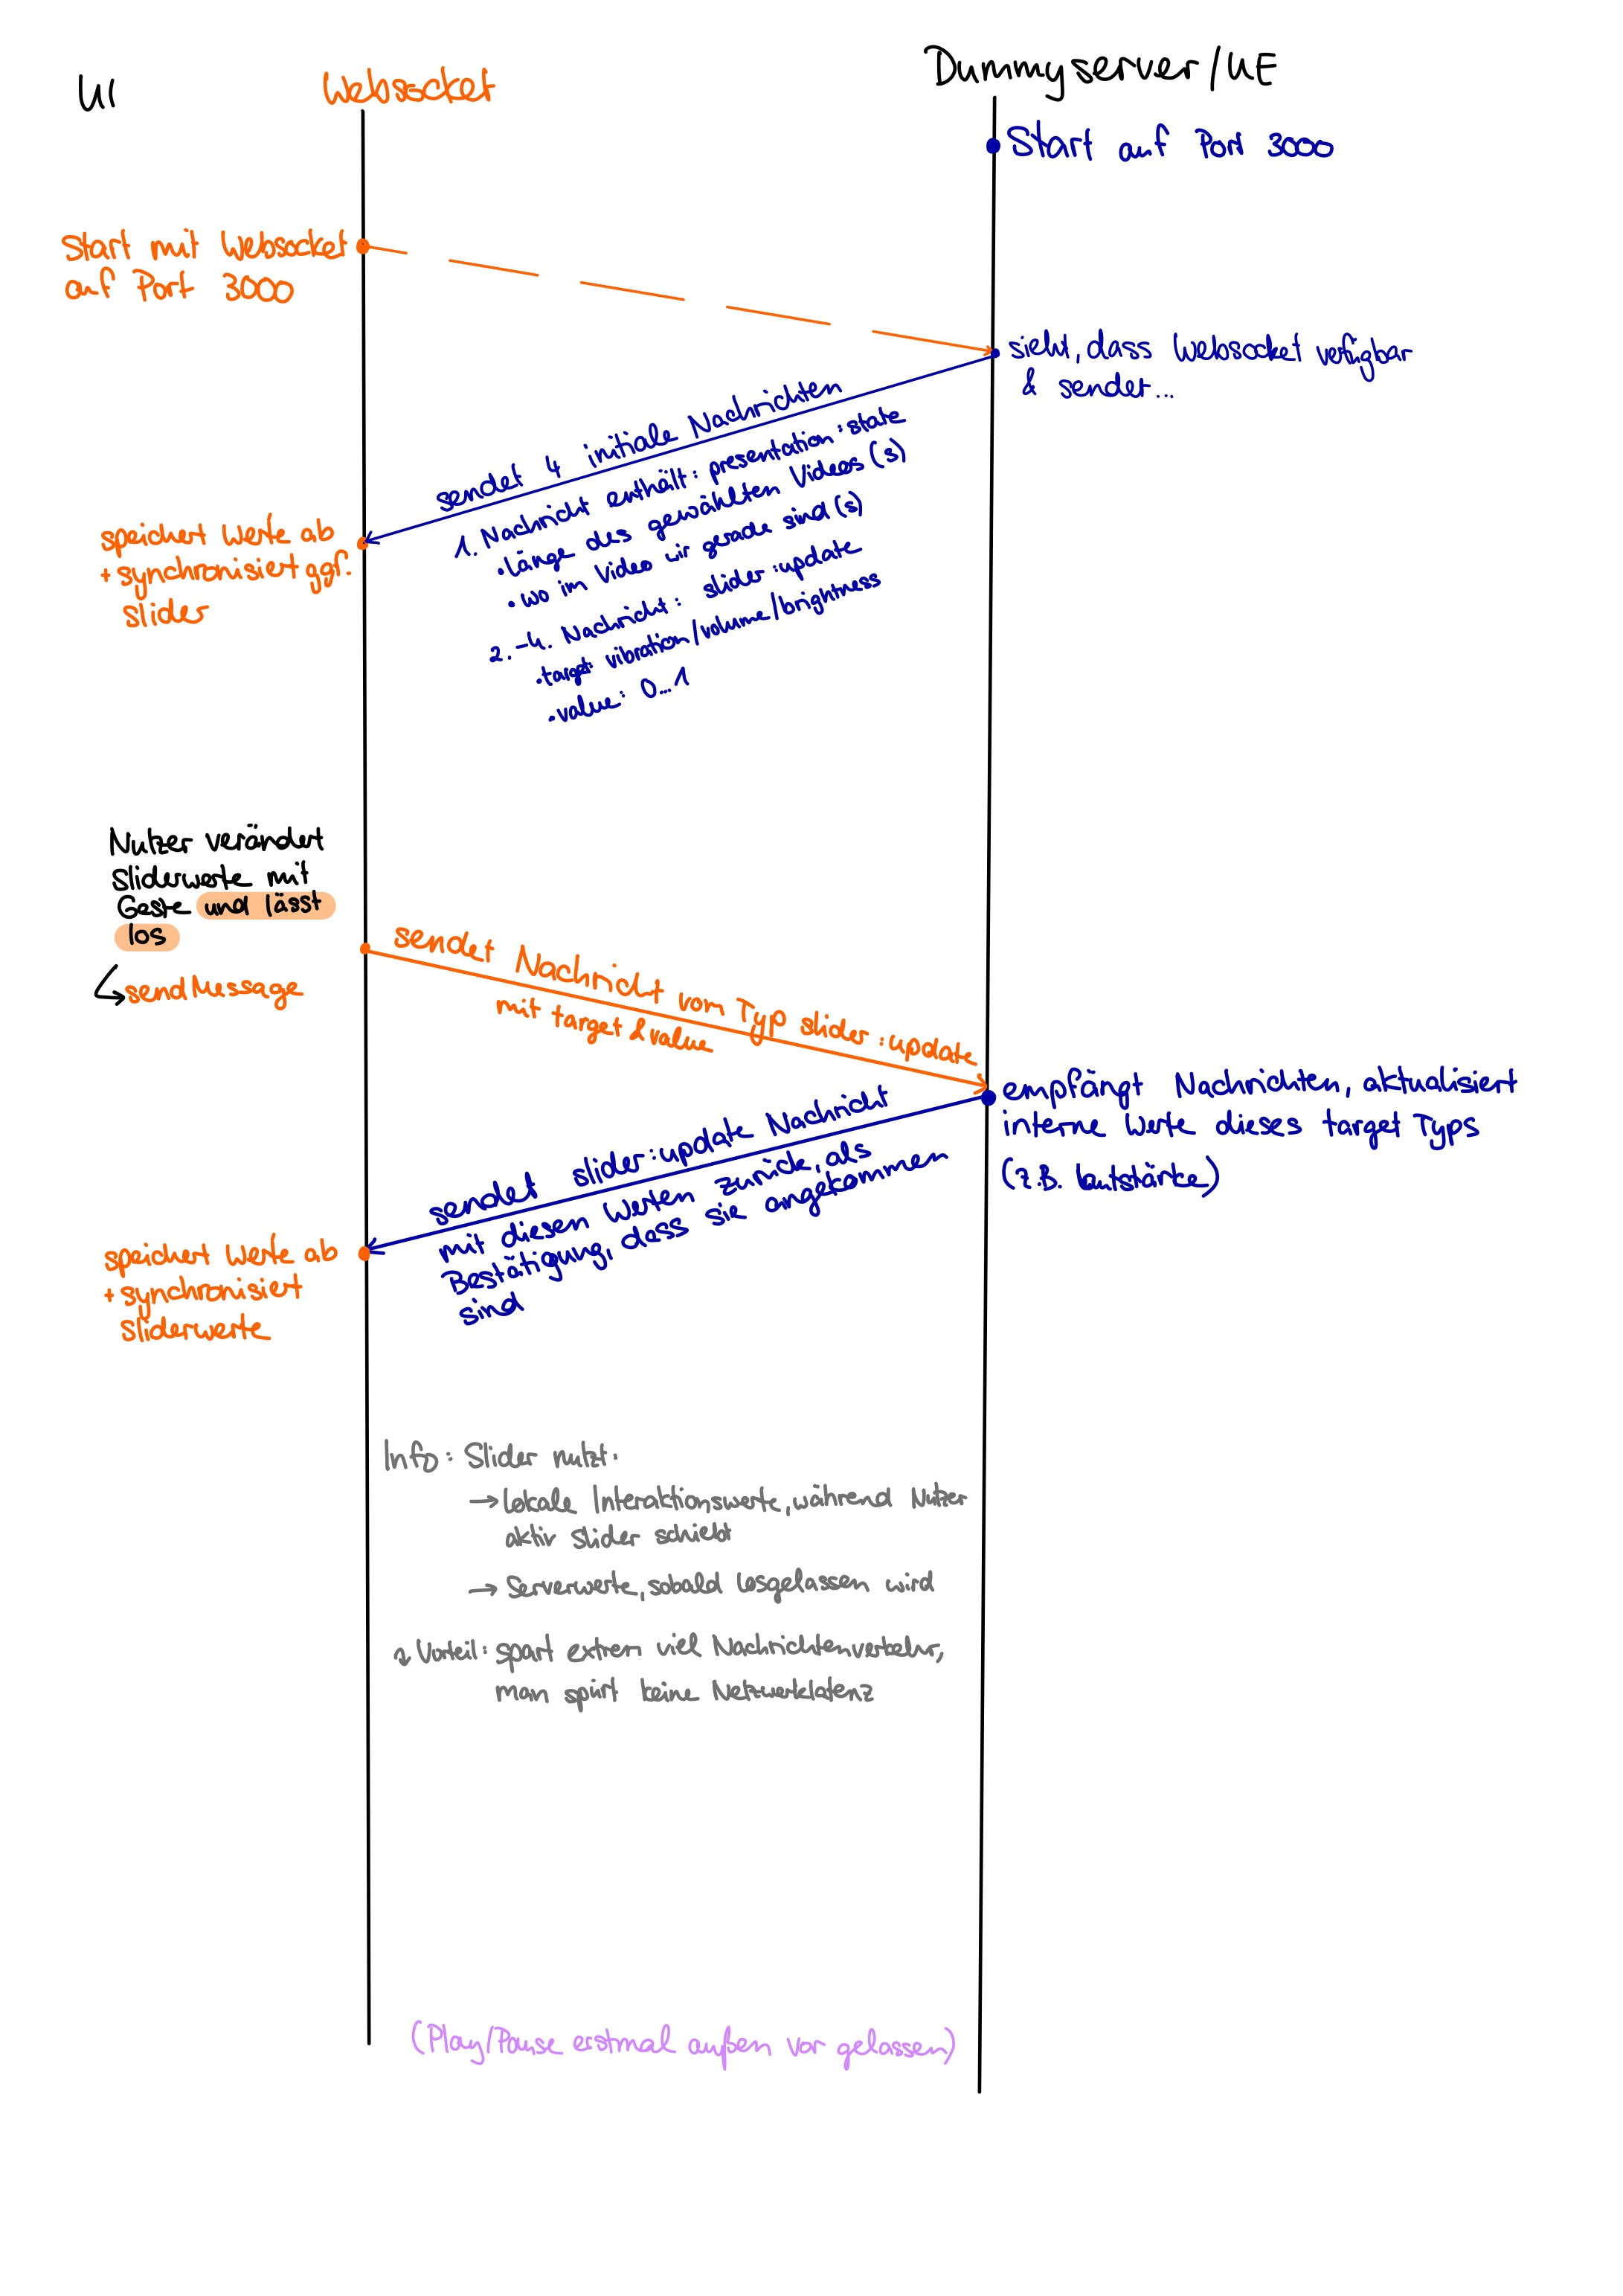
\includegraphics[width=0.9\linewidth]{content/diagrams/communication_flow.png}
\caption{Ablauf der WebSocket-basierten Eventkommunikation zwischen Overlay und Zielanwendung. Nach der Initialisierung werden Zustandsinformationen wie Menüstruktur oder Parameterwerte an das Overlay übertragen. Während der Interaktion sendet das Overlay abstrahierte Ereignisse an die Zielanwendung, welche diese verarbeitet und bei Bedarf synchronisierte Werte zur Bestätigung zurückgibt.}
\label{fig:communication_flow}
\end{figure}


\subsubsection{Anwendungsfall Präsentationssteuerung}
Für den Anwendungsfall der Präsentationssteuerung, und somit für alle Szenarien, die vorgerenderte Inhalte nutzen, ergeben sich besondere Anforderungen an die Interaktionslogik, da sowohl diskrete als auch kontinuierliche Eingaben unterstützt werden müssen.
Im Gegensatz zu reinen Menüinteraktionen kommen hierbei sowohl Button- als auch Slider-Elemente innerhalb eines Kontexts zum Einsatz.
Diese Interaktionsform wurde im Kontext der in Kapitel~\ref{sec:analyse} untersuchten atmosphärischen Szenarien mit vorgerendertem, narrativem Inhalt entwickelt, beispielsweise für die Steuerung eines Video-Mitschnitts im Fußballstadion. 
Ziel ist es, Nutzer:innen eine intuitive Kontrolle über die Wiedergabe zu ermög\-lichen, einschließlich Anhalten, Fortsetzen sowie Vor- und Zurückspulen des Materials.
Hierfür wurde ein spezieller Slider für den Zieltyp \texttt{presentation} implementiert, der, anders als die Defaultslider statt einer Prozentanzeige sowohl die Gesamtdauer des Videos als auch die aktuelle Wiedergabeposition abbildet. 
Während der Wiedergabe empfängt die Benutzungsoberfläche kontinuierlich Zeitstempel von der angebundenen Zielanwendung.
Diese werden genutzt, um den Fortschritt des Sliders dynamisch zu aktualisieren.

Ergänzend zum Slider enthält das entsprechende Menüelement eine Button-Interaktion zur Steuerung der Wiedergabe. 
Der Button schaltet zwischen den Zuständen \texttt{play} und \texttt{pause} um, und sendet entsprechend den aktuellen Status als Interaktionsereignis an die Zielanwendung.
Wird das Ende des Videos erreicht, sendet das System automatisch ein \texttt{pause}-Signal.
Bei einer erneuten Aktivierung durch die Nutzer:innen beginnt die Wiedergabe wieder am Anfang des Videos.


\subsection{Unterstützung mehrerer Projektionsflächen}
%(1) standardmäßig werden auf allen erkannten Screens electron fenster geöffnet und dann wird standard kamera auf alle gemappt
%(2) man kann im Konfigurationsmodus in electron die kamera pro bildschirm auswählen ODER im browser im Inkognito Tab pro fenster das auswählen
%(3) man kann mit modifikation von npm start command direkt bestimmte Bildschirme und bestimmte kamera mappings festlegen
%(4) es wird sichergestellt, dass bei der interaktion die aktivierungsgeste nur von der frontalen seite erkannt wird, indem abstand von kleinem finger und daumen gemessen wird (dafür wird schon vorher genutzter open Palm threshold mit offset verwendet, damit nicht noch ein parameter kalibriert werden muss - ist das überhaupt interessant?)
%(5) in browserversion werden kalibrierungskeys wahrscheinlich nicht auf alle übertragen - aber bei electron werden alle keys immer für alle bildschirme angewadnt - das ist tradeoff aber ist ja sowieso nur "gemütlichere Testvariante", also ist browser version nicht so wichtig
%(6) um electron fenster drei mal zu öffnen, aber einen webscoket zu nutzen, wird IPC angewandt. dadurch werden drei fenster als renderer von electron aufgerufen, die dann mit einer main kommunizieren und dann spricht der mein process den websocket an und macht die kommunikation mit dem Server -- alles mal vernünftig aufschreiben}

Das entwickelte Interaktionssystem wurde für den Einsatz im Multisensorischen Interaktionsraum konzipiert, in dem die Inhalte auf drei Projektionsflächen rund um die Nutzer:innen dargestellt werden.
Daraus ergibt sich die Anforderung, das Overlay nicht nur auf einem einzelnen Bildschirm, sondern parallel auf mehreren Ausgabeflächen bereitzustellen.
Das System wurde deshalb so erweitert, dass für jede relevante Projektionsfläche ein eigenes Overlay-Fenster erzeugt werden kann.
Auf diese Weise lässt sich das Marking-Menu jeweils direkt auf derjenigen Leinwand öffnen, auf der die Interaktion stattfinden soll.
In der Electron-basierten Umsetzung werden hierfür mehrere Fenster instanziiert, die jeweils als eigenständige Renderer-Prozesse ausgeführt werden.
Jedes dieser Fenster stellt ein eigenes Overlay auf einer Projektionsfläche dar, übernimmt die lokale Darstellung des Menüs und verarbeitet die zugehörigen Interaktions\-zustände.
Die übergeordnete Koordination erfolgt jedoch zentral über den Main-Prozess von Electron.
Dieser verwaltet die Kommunikation zwischen den Fenstern und bündelt zugleich die WebSocket-Kommunikation mit der angebundenen Zielanwendung.
Dadurch ist es möglich, mehrere Overlay-Fenster parallel zu betreiben, ohne für jede Projektionsfläche eine separate Netzwerkverbindung aufbauen zu müssen.
Die Kommunikation zwischen Renderer- und Main-Prozess erfolgt über \textit{Electron Inter-Process Communication (IPC)} \parencite{electronIPCdocumentation}, sodass Zustandsinformationen und Interaktionsereignisse innerhalb der Anwendung effizient verteilt werden können. Der Prozess ist in Abbildung \ref{fig:ipc_diagram} veranschaulicht.

\begin{figure}[htbp]
    \centering
    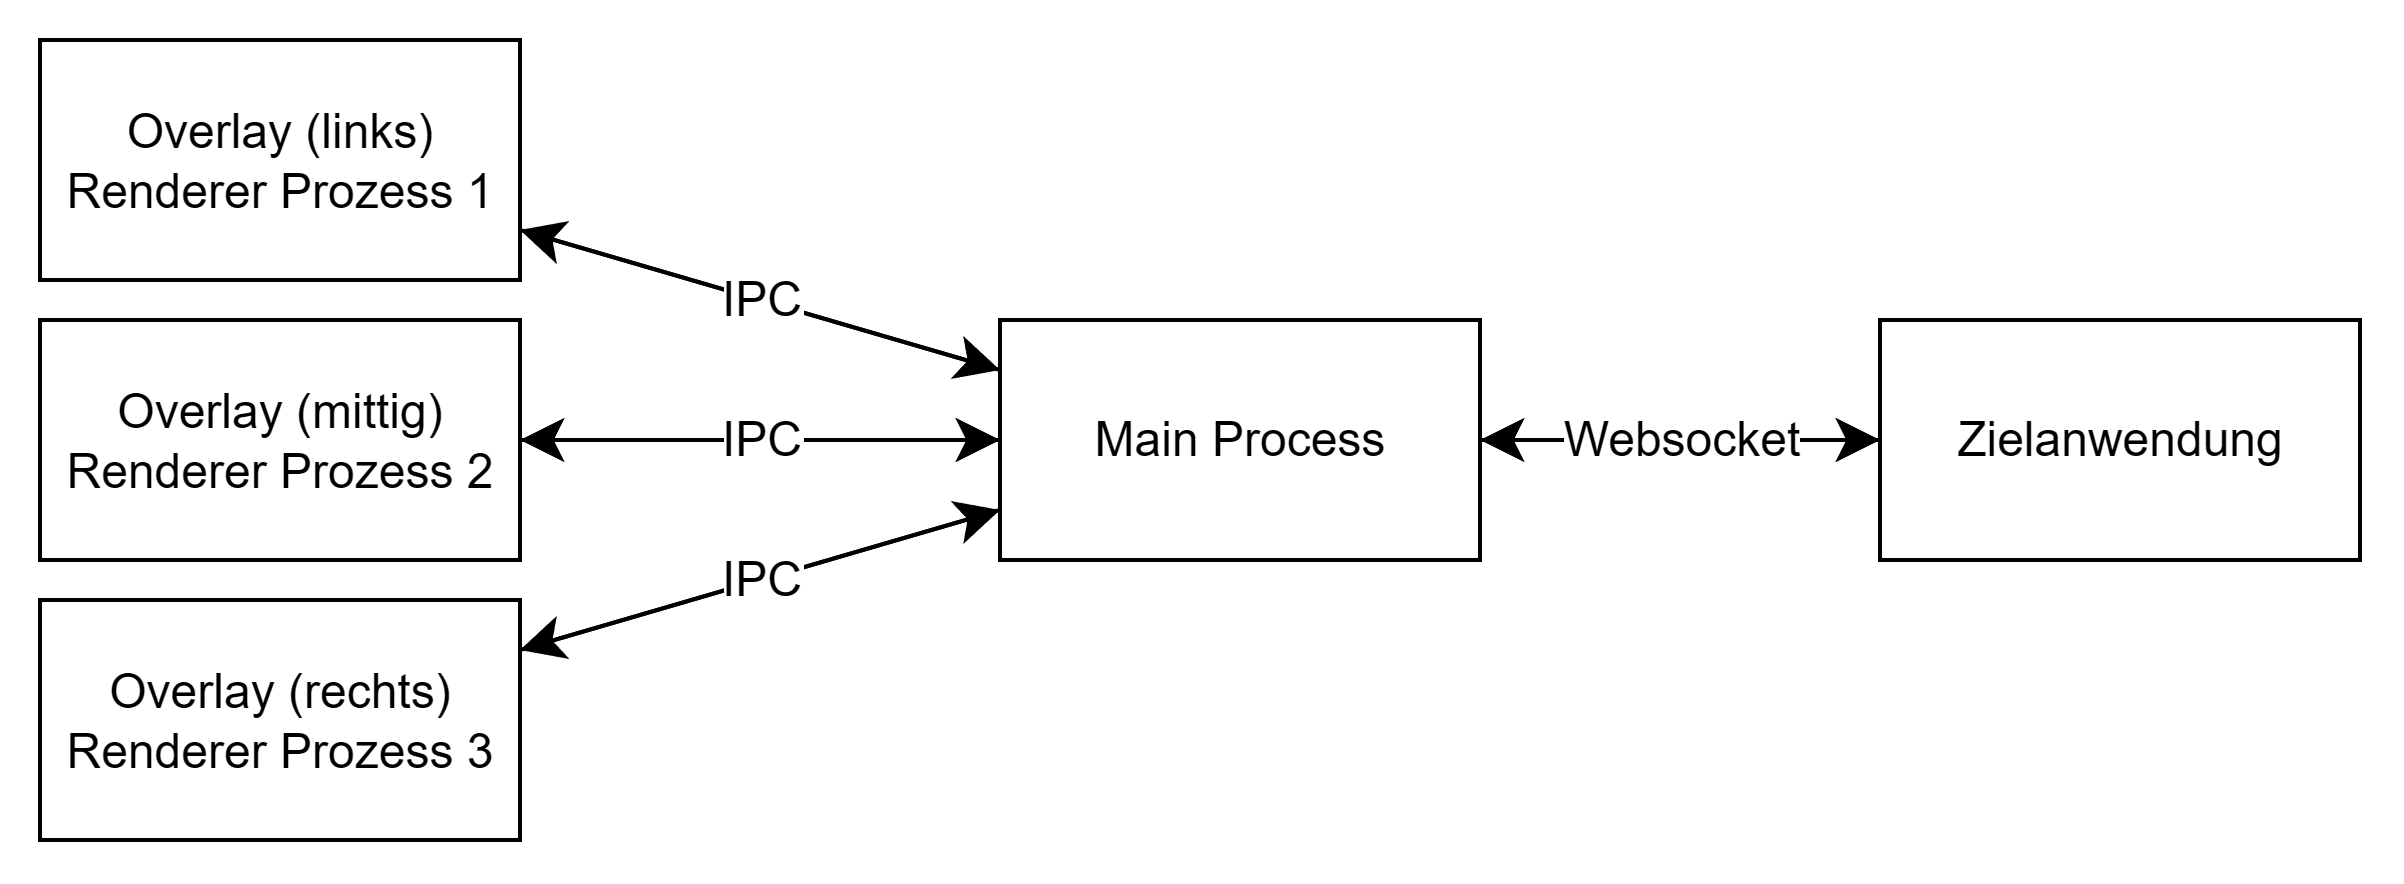
\includegraphics[width=0.9\linewidth]{content/diagrams/ipc_diagram}
    \caption{Architektur des Mehrbildschirmbetriebs. Für jede Projektionsfläche wird ein eigenes Overlay-Fenster als Renderer-Prozess erzeugt. Diese sind über Electron-IPC mit dem Main Process verbunden, der die zentrale WebSocket-Kommunikation mit der Zielanwendung übernimmt.}
    \label{fig:ipc_diagram}
\end{figure}

Eine besondere Herausforderung im Mehrbildschirmbetrieb besteht in der Zuordnung von Kameraquellen zu den jeweiligen Projektionsflächen.
Im einfachsten Fall kann dieselbe Standardkamera zunächst auf mehrere Fenster angewendet werden, um das System schnell zu starten und grundlegende Funktionen zu testen.
Für den tatsächlichen Einsatz im Interaktionsraum ist jedoch eine gezielte Zuordnung erforderlich, da für jede Leinwand eine Kamera zur Verfügung steht. Dafür wurden mehrere Konfigurationsmöglichkeiten vorgesehen. Zum einen kann im Konfigurationsmodus innerhalb des Overlays eine Kamera auf jedem Bildschirm ausgewählt werden (siehe Abbildung \ref{fig:select_kamera_interface}).
Zum anderen lässt sich in der browserbasierten Variante die gewünschte Kamera direkt im jeweiligen Fenster festlegen. Zusätzlich besteht die Möglichkeit, beim Start der Anwendung feste Zuordnungen von Bildschirmen und Kameras über Startparameter vorzugeben. Diese unterschiedlichen Konfigurationswege erleichtern sowohl das flexible Testen als auch den reproduzierbaren Einsatz in der Zielumgebung.

\begin{figure}[htbp]
    \centering
    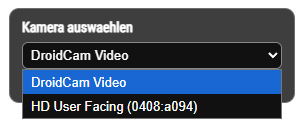
\includegraphics[width=0.6\linewidth]{content/images/select_kamera_interface}
    \caption{Benutzungsoberfläche, die im Konfigurationsmodus auf jedem aktiven Bildschirm angezeigt wird, um die zugehörige Kamera auszuwählen.}
    \label{fig:select_kamera_interface}
\end{figure}

Damit eine Interaktion nur auf der jeweils passenden Leinwand ausgelöst wird, muss das System sicherstellen, dass Aktivierungsgesten nicht gleichzeitig oder versehentlich auf mehreren Projektionsflächen interpretiert werden.
Dies ist insbesondere dann relevant, wenn eine Hand von mehreren Kameras teilweise erfasst wird. Zur Reduktion solcher Fehlaktivierungen wurde die Aktivierungsgeste so definiert, dass sie nur bei einer ausreichend frontalen Handausrichtung erkannt wird. Hierzu wird neben den allgemeinen Merkmalen der offenen Hand zusätzlich die relative Anordnung ausgewählter Landmarken berücksichtigt. Insbesondere der Abstand zwischen Daumen und kleinem Finger wird genutzt, um abzuschätzen, ob die Handfläche zur Kamera orientiert ist (siehe Abbildung \ref{fig:hand_frontal_site}). Dadurch wird erreicht, dass das Menü bevorzugt auf derjenigen Leinwand aktiviert wird, vor der die Nutzer:innen tatsächlich stehen, während seitlich erfasste Hände die Aktivierung nicht oder nur deutlich seltener auslösen.

\begin{figure}[htbp]
    \centering
    \begin{subfigure}[t]{0.32\textwidth}
        \centering
        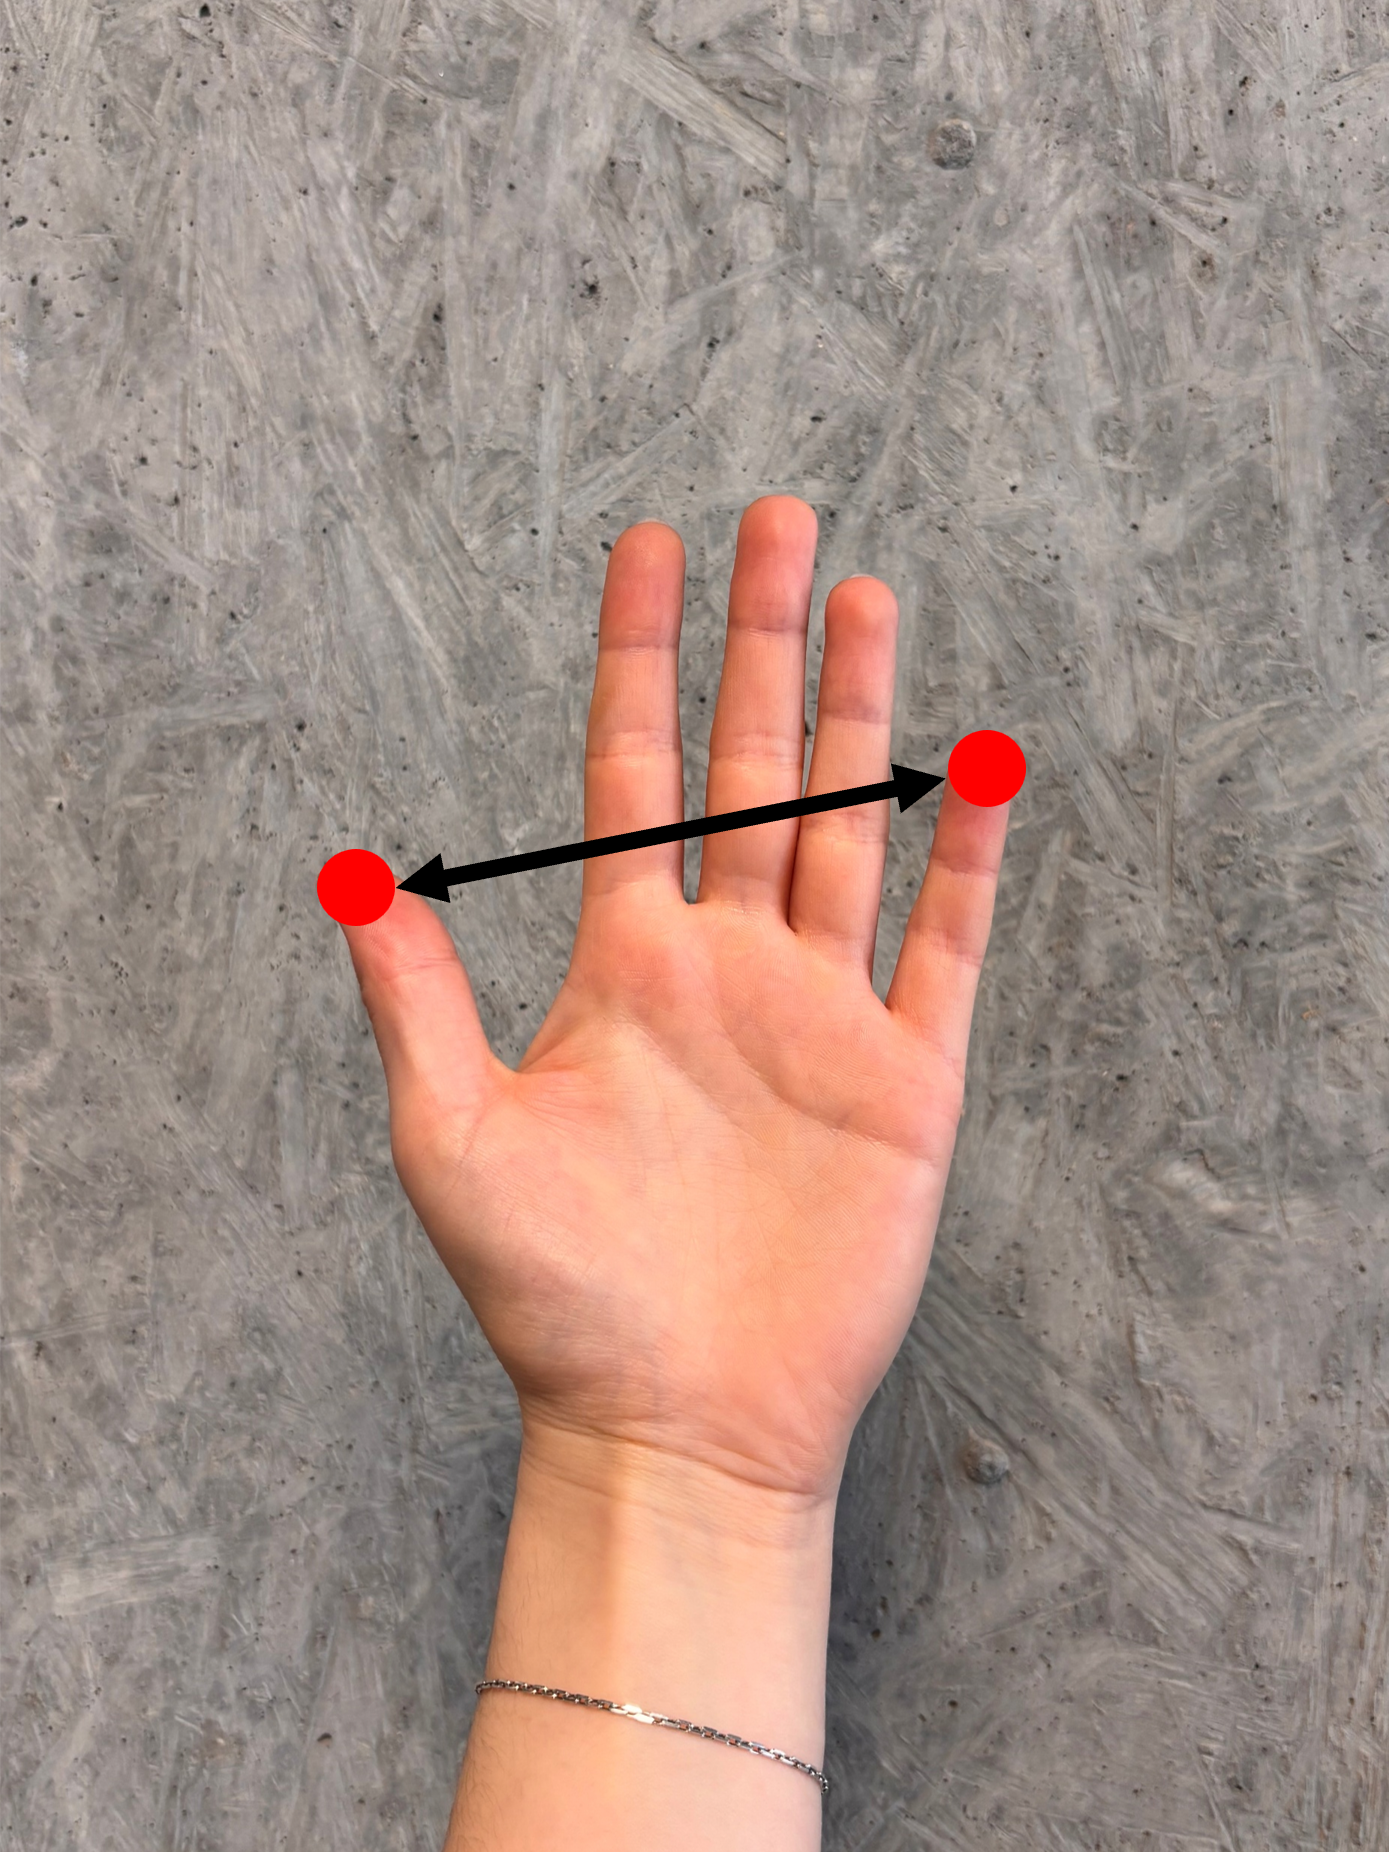
\includegraphics[width=\linewidth]{content/images/hand_frontal.png}
        \caption{Aktivierungsgeste wird erkannt.}
        \label{fig:hand_frontal}
    \end{subfigure}
    \hfill
    \begin{subfigure}[t]{0.32\textwidth}
        \centering
        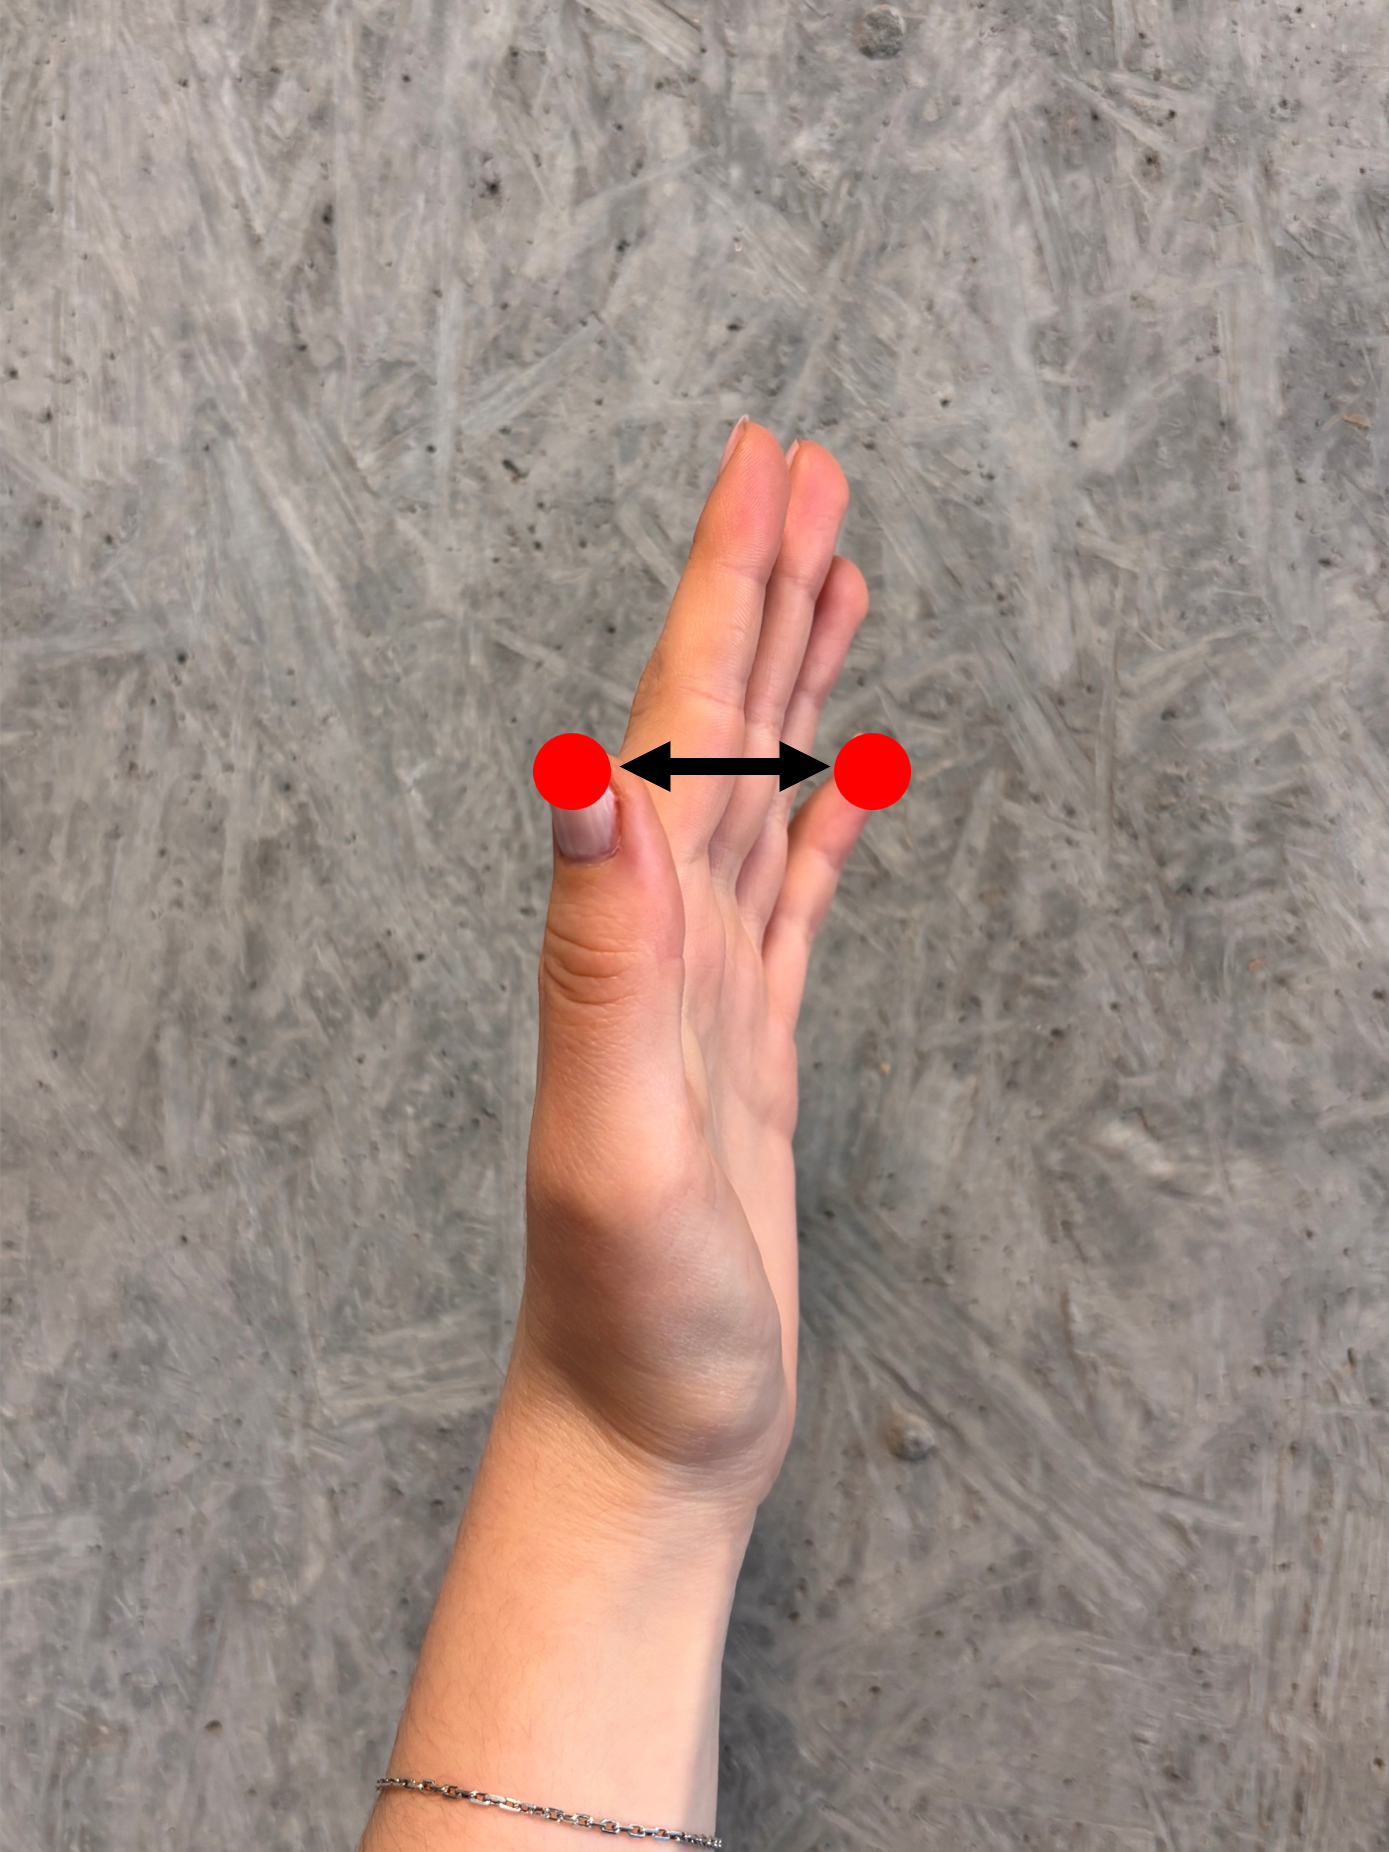
\includegraphics[width=\linewidth]{content/images/hand_half_frontal.png}
        \caption{Aktivierungsgeste wird aus dieser Perspektive nicht erkannt.}
        \label{fig:hand_half_frontal}
    \end{subfigure}
    \hfill
    \begin{subfigure}[t]{0.32\textwidth}
        \centering
        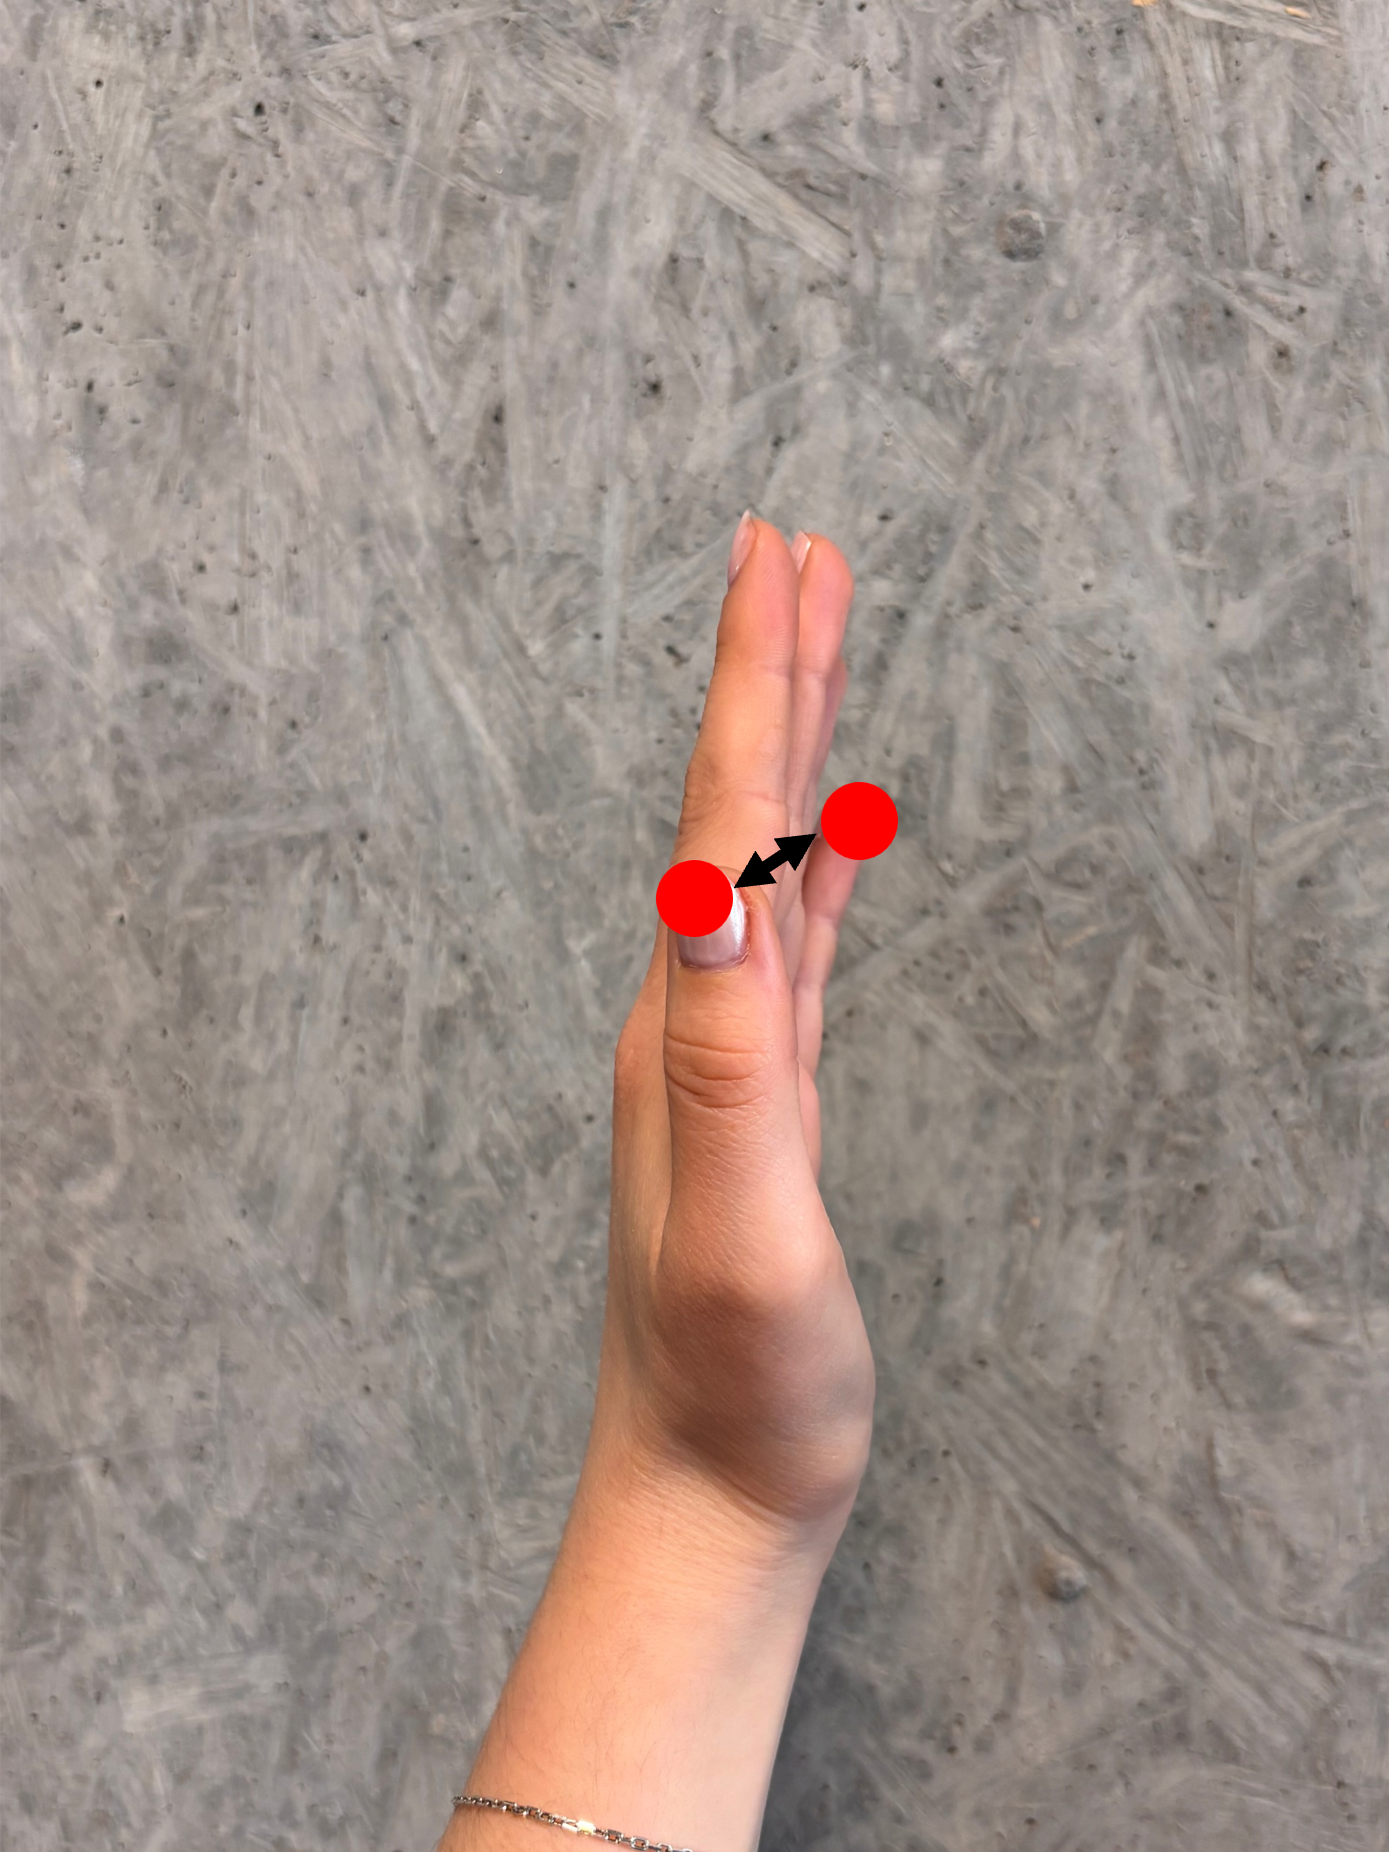
\includegraphics[width=\linewidth]{content/images/hand_site.png}
        \caption{Aktivierungsgeste wird aus dieser Perspektive nicht erkannt.}
        \label{fig:hand_site}
    \end{subfigure}
    \caption{Handorientierung: gültige und ungültige Aktivierungsgeste}
    \label{fig:hand_frontal_site}
\end{figure}

Die Mehrbildschirmarchitektur erweitert das Interaktionssystem somit um eine räumliche Dimension.
Das Overlay ist nicht mehr auf einen einzelnen Anzeigekontext beschränkt, sondern kann als verteilte Interaktionsschicht innerhalb des gesamten Multisensorischen Interaktionsraums eingesetzt werden. Gleichzeitig bleibt die grundlegende Systemarchitektur erhalten: Handtracking, Interaktionslogik, Darstellung und Zielanwendung bleiben voneinander getrennt. Dadurch kann das System auch im Mehrbildschirmbetrieb modular konfiguriert, getestet und an unterschiedliche räumliche Setups angepasst werden.


\subsection{Entwicklungs- und Testumgebung}
\label{sec:development}
Zur Unterstützung der Implementierung wurden mehrere Werkzeuge eingesetzt, die insbesondere die Entwicklung, das Testen und das Debugging des Interaktionssystems erleichtern sollen.
Eine zentrale Rolle spielte dabei ein Mock-Server, der das Verhalten einer Zielanwendung simuliert. Dieser Server stellt initiale Menü- und Statusdaten bereit, verarbeitet eingehende Interaktionsnachrichten des Overlays und sendet entsprechende Zustandswerte zurück. Dadurch konnte die Kommunikationsschnittstelle unabhängig von einer laufenden Zielanwendung entwickelt und getestet werden.

Zusätzlich wurde ein Offline-Modus vorgesehen, in dem das System mit lokalen Testdaten arbeitet. Dadurch kann die Benutzungsoberfläche auch ohne aktive WebSocket-Verbindung betrieben werden, was isolierte Tests einzelner Komponenten ermöglicht. Dafür wurde das System zusätzlich als browserbasierte Variante bereitgestellt, wodurch eine einfache Demonstration und ein schneller Zugriff auf das Interaktionssystem ohne lokale Installation möglich wurde.

Ergänzend zu Mock-Server und Offline-Modus wurde das Interaktionssystem bereits exemplarisch an eine konkrete Testanwendung durch einen Entwickler des MIR angebunden. Dabei wurden vorgerenderte Videoinhalte über die entwickelte WebSocket-Schnittstelle gesteuert. Als Testfall diente unter anderem ein kurzes Video einer Berglandschaft, das sich aufgrund seiner geringen Länge besonders für wiederholte Tests der Wiedergabe- und Timeline-Steuerung eignete. Über das Marking-Menu konnten dabei sowohl die Lautstärke als auch der Wiedergabezustand sowie das Vor- und Zurückspulen des Videos gesteuert werden. Da dieses Testszenario nicht Bestandteil der in Abschnitt~\ref{sec:analyse} untersuchten Szenarien war, diente es primär der technischen Überprüfung der Anbindung.
Abbildung~\ref{fig:berg_testanwendung} zeigt beispielhaft die angebundene Testanwendung im MIR.

\begin{figure}[H]
    \centering
    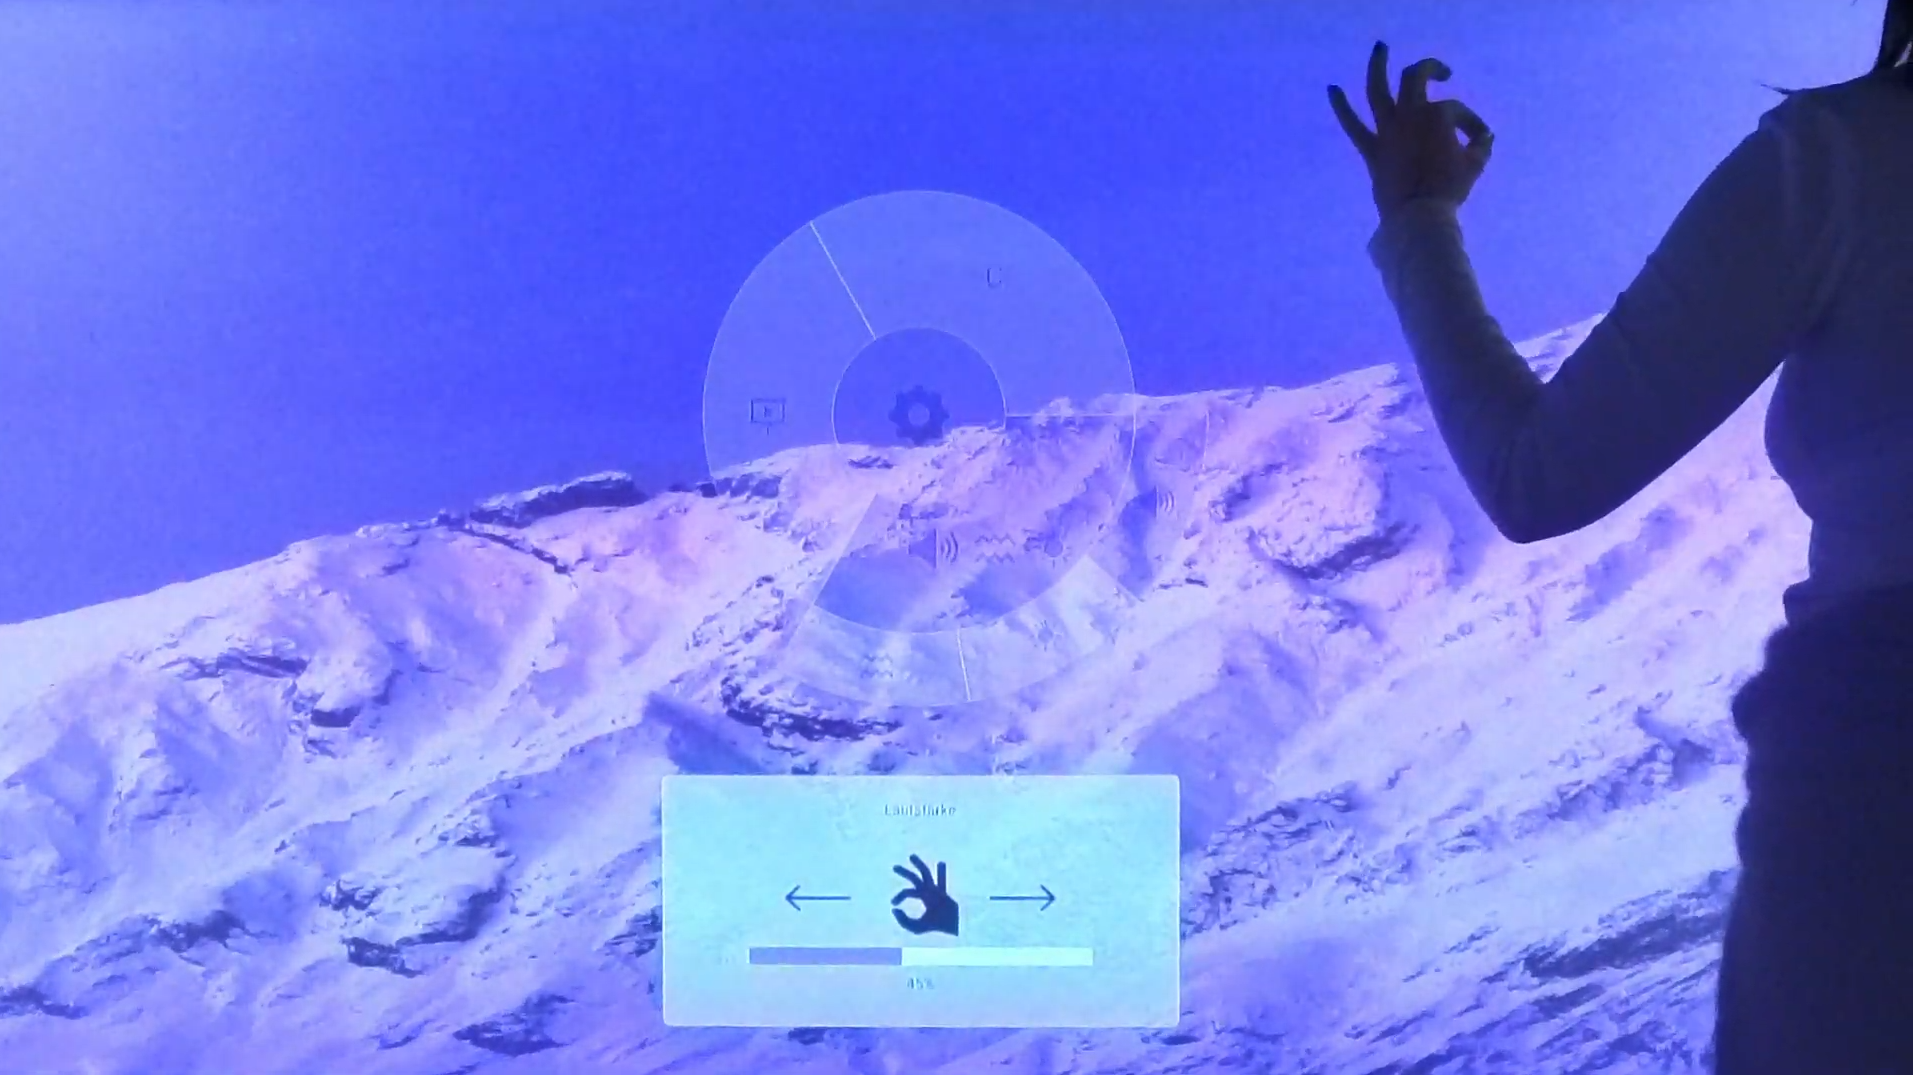
\includegraphics[width=0.8\linewidth]{content/images/vieo-still.png}
    \caption{Ausschnitt aus einem Interaktionsvideo des Berglandschaftsszenarios mit vorgerendertem Videoinhalt. Die Umgebung wird durch eine Nutzerin über das Marking-Menu gesteuert.}
    \label{fig:berg_testanwendung}
\end{figure}

Neben diesen angebundenen Tests erfolgte ein Großteil der Entwicklung auf einem Laptop-System, während Tests des vollständigen Interaktionssystems im Multisensorischen Interaktionsraum durchgeführt wurden. Da die Größe und Position des Marking-Menus auf den großflächigen Projektionen deutlich anders wahrgenommen werden als auf einem Laptopdisplay, wurden zusätz\-liche Kalibrierungsfunktionen implementiert.
Über Tastaturkürzel konnten während der Ent\-wick\-lungs\-phase Parameter wie die Position, Skalierung und Darstellung des Menüs angepasst werden. Ebenso konnten Schwellwerte der Gestenerkennung sowie Dwell-Zeiten zur Interaktionsauslösung dynamisch verändert werden. Diese Funktionen erleichterten die Feinabstimmung des Interaktionssystems in unterschiedlichen Testumgebungen.

Diese Werkzeuge unterstützten insbesondere die iterative Entwicklung und ermöglichten eine schrittweise Überprüfung der einzelnen Systemkomponenten. Die Tests wurden dabei nicht ausschließlich isoliert durchgeführt, sondern erfolgten auch im Multisensorischen Interaktionsraum in Zusammenarbeit mit einem Entwickler des Systems sowie dem Betreuer der Arbeit. Dadurch konnten praktische Aspekte der Integration und Nutzung frühzeitig berücksichtigt werden.


\subsection{Integration der Systemkomponenten}
Die beschriebenen Komponenten bilden gemeinsam das entwickelte Interaktionssystem für den Multisensorischen Interaktionsraum. 
Das Handtracking liefert kontinuierlich Handlandmarkeninformationen der Nutzer:innen, aus denen Cursorbewegungen und Interaktions\-zustände abgeleitet werden.
Diese Informationen steuern das im Electron-Overlay dargestellte Marking-Menu sowie dessen Interaktionslogik.
Über die WebSocket-Schnittstelle werden Interaktionsereignisse an die angebundene Zielanwendung übertragen und mit deren Zustand synchronisiert. 
Die datengetriebene Menüstruktur ermöglicht es dabei, die Interaktionsoberfläche flexibel an unterschiedliche Anwendungsszenarien anzupassen.
Durch die modulare Architektur bleiben Tracking, Benutzungsoberfläche und Zielanwendung voneinander getrennt, wodurch das System flexibel an unterschiedliche Anwendungsszenarien angepasst werden kann.

Das entwickelte System stellt damit eine prototypische Umsetzung körper\-basierter Interaktion im MIR dar, die als Grundlage für zukünftige Erweiterungen und Anwendungsszenarien dienen kann.